
%%
%% forked from https://gits-15.sys.kth.se/giampi/kthlatex kthlatex-0.2rc4 on 2020-02-13
%% expanded upon by Gerald Q. Maguire Jr.
%% This template has been adapted by Anders Sjögren to the University
%% Engineering Program in Computer Science at KTH ICT. Adaptation is the
%% translation of English headings into Swedish as the addition of Swedish
%% text. Original body text is deliberately left in English.

%% Conventions for todo notes:
% \todo[inline]{Comments/directions/... in English}
% \todo[inline, backgroundcolor=kth-lightblue40]{Text på svenska}
% \todo[inline, backgroundcolor=kth-lightgreen40]{English descriptions about formatting}
% \todo[inline, backgroundcolor=kth-lightred40]{warnings}

%% The template is designed to handle a thesis in English or Swedish
% set the default language to english or swedish by passing an option to the documentclass - this handles the inside tile page
% To optimize for digital output (this changes the color palette add the option: digitaloutput
% To use bibtex or biblatex - include one of these as an option
\documentclass[english, bibtex]{kththesis}
%\documentclass[swedish, biblatex]{kththesis}

% \usepackage[style=numeric,sorting=none,backend=biber]{biblatex}
\ifbiblatex
    %\usepackage[language=english,bibstyle=authoryear,citestyle=authoryear, maxbibnames=99]{biblatex}
    \usepackage[bibstyle=authoryear,citestyle=authoryear, maxbibnames=99,language=english]{biblatex}
    % alternatively you might use another style, such as IEEE
    %\usepackage[style=ieee]{biblatex}
    \addbibresource{references.bib}
    %\DeclareLanguageMapping{norsk}{norwegian}
\else
    % The line(s) below are for BibTeX
    \bibliographystyle{bibstyle/myIEEEtran}
    %\bibliographystyle{apalike}
\fi


% include a variety of packages that are useful
%%%%%%%%%%%%%%%%%%%%%%%%%%%%%% Packages %%%%%%%%%%%%%%%%%%%%%%%%%%%%%%
% The following is for use with the KTH cover when not using XeLaTeX or LuaLaTeX
\ifxeorlua\relax
\else
\usepackage[scaled]{helvet}
\fi

%% The following are needed for generating the DiVA page(s)
\usepackage[force-eol=true]{scontents}              %% Needed to save lang, abstract, and keywords
\usepackage{pgffor}                 %% includes the foreach loop

%% Basic packages

%% Links
\usepackage{xurl}                %% Support for breaking URLs

%% Colorize
%\usepackage{color}
\PassOptionsToPackage{dvipsnames, svgnames}{xcolor}
\usepackage{xcolor}

\usepackage[normalem]{ulem}
\usepackage{soul}
\usepackage{xspace}
\usepackage{braket}

% to support units and decimal aligned columns in tables
\usepackage[locale=US]{siunitx}

\usepackage{balance}
\usepackage{stmaryrd}
\usepackage{booktabs}
\usepackage{graphicx}	        %% Support for images
\usepackage{multirow}	        %% Support for multirow columns in tables
\usepackage{tabularx}		    %% For simple table stretching
\usepackage{mathtools}
\usepackage{algorithm} 
\usepackage{algorithmic}  
\usepackage{amsmath}
\usepackage[linesnumbered,ruled,vlined,algo2e]{algorithm2e}
% can't use both algpseudocode and algorithmic packages
%\usepackage[noend]{algpseudocode}
%\usepackage{subfig}  %% cannot use both subcaption and subfig packages
\usepackage{optidef}
\usepackage{float}		        %% Support for more flexible floating box positioning
\usepackage{pifont}

%% some additional useful packages
% to enable rotated figures
\usepackage{rotating}	    	%% For text rotating
\usepackage{array}		        %% For table wrapping
\usepackage{mdwlist}            %% various list-related commands
\usepackage{setspace}           %% For fine-grained control over line spacing


\usepackage{enumitem}           %% to allow changes to the margins of descriptions


%% If you are going to include source code (or code snippets)
\usepackage{listings}		    %% For source code listing
%%\usepackage[cache=false]{minted} %% For source code highlighting
%%\usemintedstyle{borland}

\usepackage{bytefield}          %% For packet drawings


\setlength {\marginparwidth }{2cm} %leave some extra space for todo notes
\usepackage{todonotes}
\usepackage{notoccite} % do not number captions based on their appearance in the TOC


% Footnotes
\usepackage{perpage}
\usepackage[perpage,para,symbol]{footmisc} %% use symbols to ``number'' footnotes and reset which symbol is used first on each page


%% Various useful packages
%%----------------------------------------------------------------------------
%%   pcap2tex stuff
%%----------------------------------------------------------------------------
\usepackage{tikz}
\usepackage{colortbl}
\usetikzlibrary{arrows,decorations.pathmorphing,backgrounds,fit,positioning,calc,shapes}
\usepackage{pgfmath}	% --math engine
\newcommand\bmmax{2}
\usepackage{bm} % bold math


%% Managing titles
% \usepackage[outermarks]{titlesec}
%%%%%%%%%%%%%%%%%%%%%%%%%%%%%%%%%%%%%%%%%%%%%%%%%%%%%%%%%%%%%%%%%%%%%%
%\captionsetup[subfloat]{listofformat=parens}

% to include PDF pages
%\usepackage{pdfpages}


\usepackage{csquotes}               %% Recommended by biblatex
% to provide a float barrier use:
\usepackage{placeins}

\usepackage{comment}  %% Provides a comment environment
\usepackage{refcount}   %% to be able to get an expandable \getpagerefnumber

% for experiments with new cover
\usepackage{eso-pic}
\usepackage[absolute,overlay]{textpos}

% when the package is used, it draws boxes on the page showing the text, footnote, header, and margin regions of the page
%\usepackage{showframe}  
%\usepackage{printlen} % defines the printlength command to print out values of latex variable

\usepackage{xparse}  % to use for commands with optional arguments

%%% Local Variables:
%%% mode: latex
%%% TeX-master: t
%%% End:
% KTH colors for LaTeX documents
%
% Started from kthcolors by:
% Riccardo Sven Risuleo
% 2016-09-06 11:05:40
%
% from https://github.com/KTH-AC/kthcolors
%
% Adapted using the colors from "Graphic Profile Manual KTH" version 180604
% (i.e.. 2018-06-04) 
% see https://intra.kth.se/en/administration/kommunikation/grafiskprofil/kth-s-grafiska-profil-1.844676
% 
% G. Q. Maguire Jr.
% 2021-07-05
%

%\NeedsTexFormat{LaTeX2e}[1994/06/01]
%\ProvidesPackage{kthcolors}[2021/07/85 v3 Latex package with official KTH colors]

\RequirePackage{xcolor}
%% Primary colors
%% As of the new manual, there is only 1 primary color; but with three 
\definecolor{kth-blue}{RGB/cmyk}{25,84,166/0.849,0.494,0,0.349}
\colorlet{kth-blue80}{kth-blue!80!}
\colorlet{kth-blue40}{kth-blue!40!}

% these are no longer used as of 2018-06-04
%\definecolor{kth-red}{RGB/cmyk}{157,16,45/0,0.898,0.713,0.384}
%\definecolor{kth-green}{RGB/cmyk}{98,146,46/0.329,0,0.685,0.427}

%% Secondary colors
\definecolor{kth-lightblue}{RGB/cmyk}{36,160,216/0.833,0.259,0,0.153}
\colorlet{kth-lightblue80}{kth-lightblue!80!}
\colorlet{kth-lightblue40}{kth-lightblue!40!}

%\definecolor{kth-lightred}{RGB/cmyk}{228,54,62/0,0.763,0.728,0.106}
\definecolor{kth-lightred}{RGB}{216,84,151}
\colorlet{kth-lightred80}{kth-lightred!80!}
\colorlet{kth-lightred40}{kth-lightred!40!}

\definecolor{kth-lightgreen}{RGB/cmyk}{176,201,43/0.124,0,0.786,0.212} % olive
\colorlet{kth-lightgreen80}{kth-lightgreen!80!}
\colorlet{kth-lightgreen40}{kth-lightgreen!40!}

% Cool Gray 9C
%\definecolor{kth-coolgray}{RGB}{101,101,108}

% Cool Gray 10 suggested by Martin Krzywinski (see http://mkweb.bcgsc.ca/colorblind) 
\definecolor{kth-coolgray}{RGB}{99,102,106}
\colorlet{kth-coolgray80}{kth-coolgray!80!}
\colorlet{kth-coolgray40}{kth-coolgray!40!}

% Tertiary colors (yet more colors)
% All of these are no longer used
%\definecolor{kth-pink}{RGB/cmyk}{216,84,151/10,0.611,0.301,0.153}
%\definecolor{kth-yellow}{RGB/cmyk}{250,185,25/0,0.26,0.9,0.0196}
%\definecolor{kth-darkgray}{RGB/cmyk}{101,101,108/0.0648,0.0648,0,0.576}
%\definecolor{kth-middlegray}{RGB/cmyk}{189,188,188/0,0.00529,0.00529,0.259}
%\definecolor{kth-lightgray}{RGB/cmyk}{227,229,227/0.00873,0,0.00873,0.102}

%\DeclareOption{gray}{\colorlet{gray}{kth-darkgray}}

% These versions are designed to meet accessability requirements for digital media
% Note that the palette is more limited than for the print version of the colors
\ifdigitaloutput
    % primary color
    \definecolor{kth-blue}{HTML}{1954A6} % Deep sea
    \definecolor{kth-blue80}{HTML}{5E87C0}

    % Secondary colors
    \definecolor{kth-lightblue}{HTML}{2191C4} % Stratosphere
    \definecolor{kth-lightred}{HTML}{D02F80} % Fluorescence
    \definecolor{kth-lightred80}{HTML}{D95599}
    \definecolor{kth-lightgreen}{HTML}{62922E} % Front-lawn
    \definecolor{kth-coolgray}{HTML}{65656C} % Office
    \definecolor{kth-coolgray80}{HTML}{848489}
\fi



%\glsdisablehyper
%\makeglossaries
%\makenoidxglossaries
%%%% Local Variables:
%%% mode: latex
%%% TeX-master: t
%%% End:

% The form of the entries in this file is \newacronym{label}{acronym}{phrase}
%                                      or \newacronym[options]{label}{acronym}{phrase}
% see "User Manual for glossaries.sty" for the  details about the options, one example is shown below
% note the specification of the long form plural in the line below
\newacronym[longplural={Debugging Information Entities}]{DIE}{DIE}{Debugging Information Entity}
%
% The following example also uses options
\newacronym[plural={OSes}, firstplural={operating systems (OSes)}]{OS}{OS}{operating system}

% note the use of a non-breaking dash in long text for the following acronym
\newacronym{IQL}{IQL}{Independent Q‑Learning}

\newacronym{KTH}{KTH}{KTH Royal Institute of Technology}

\newacronym{LAN}{LAN}{Local Area Network}
% note the use of a non-breaking dash in the following acronym
\newacronym{WiFi}{Wi-Fi}{Wireless Fidelity}

\newacronym{WLAN}{WLAN}{Wireless Local Area Network}
\newacronym{UN}{UN}{United Nations}
\newacronym{SDG}{SDG}{Sustainable Development Goal}
                %load the acronyms file

\makeatletter
\newcommand{\DeclareLatinAbbrev}[2]{%
  \DeclareRobustCommand{#1}{%
    \@ifnextchar{.}{\textit{#2}}{%
      \@ifnextchar{,}{\textit{#2.}}{%
        \@ifnextchar{!}{\textit{#2.}}{%
          \@ifnextchar{?}{\textit{#2.}}{%
            \@ifnextchar{)}{\textit{#2.}}{%
              {\textit{#2.,\ }}}}}}}}%
}
\makeatother
\DeclareLatinAbbrev{\eg}{e.g}
\DeclareLatinAbbrev{\Eg}{E.g}
\DeclareLatinAbbrev{\ie}{i.e}
\DeclareLatinAbbrev{\Ie}{I.e}
\DeclareLatinAbbrev{\etc}{etc}
\DeclareLatinAbbrev{\etal}{et~al}

\def\first {$(i)$\xspace}
\def\second{$(ii)$\xspace}
\def\third {$(iii)$\xspace}
\def\fourth{$(iv)$\xspace}
\def\fifth {$(v)$\xspace}
\def\sixth {$(vi)$\xspace}
\def\seventh{$(vii)$\xspace}
\def\eighth{$(viii)$\xspace}

%%% custom definitions
%% Coloring the links!
\newcommand\myshade{75} % Usage: red!\myshade!black

\definecolor{ForestGreen} {RGB}{34,  139,  34}
\definecolor{HeraldRed2}   {rgb}{0.81, 0.12, 0.15}

\newcommand{\refscolor} {blue}
\newcommand{\linkscolor}{HeraldRed2}
\newcommand{\urlscolor} {ForestGreen}

%% Some definitions of used colors
%\definecolor{darkblue}{rgb}{0.0,0.0,0.3} %% define a color called darkblue
%\definecolor{darkred}{rgb}{0.4,0.0,0.0}
%\definecolor{red}{rgb}{0.7,0.0,0.0}
%\definecolor{lightgrey}{rgb}{0.8,0.8,0.8} 
%\definecolor{grey}{rgb}{0.6,0.6,0.6}
%\definecolor{darkgrey}{rgb}{0.4,0.4,0.4}
%\definecolor{aqua}{rgb}{0.0, 1.0, 1.0}

% For runin headings
\newcommand{\smartparagraph}[1]{\vspace{.05in}\noindent\textbf{#1}}

%% Table of Contents (ToC) depth 
\setcounter{secnumdepth}{4} % how many sectioning levels to assign numbers to
\setcounter{tocdepth}{4}    % how many sectioning levels to show in ToC

%% Limit hyphenation
\hyphenpenalty=9000
\tolerance=5000
% Reduce hyphenation as much as possible:
%\hyphenpenalty=15000
%\tolerance=1000

% For notes by the authors to themselves
\newcommand*{\todoinline}[1]{\textcolor{red}{TODO: #1}}

  % load some additional definitions to make writing more consistent

% The following is needed in conjunction with generating the DiVA data with abstracts and keywords using the scontents package and a modified listings environment
%\usepackage{listings}   %  already included
\ExplSyntaxOn
\newcommand\typestoredx[2]{\expandafter\__scontents_typestored_internal:nn\expandafter{#1} {#2}}
\ExplSyntaxOff
\makeatletter
\let\verbatimsc\@undefined
\let\endverbatimsc\@undefined
\lst@AddToHook{Init}{\hyphenpenalty=50\relax}
\makeatother


\lstnewenvironment{verbatimsc}
    {
    \lstset{%
        basicstyle=\ttfamily\tiny,
        backgroundcolor=\color{white},
        %basicstyle=\tiny,
        %columns=fullflexible,
        columns=[l]fixed,
        language=[LaTeX]TeX,
        %numbers=left,
        %numberstyle=\tiny\color{gray},
        keywordstyle=\color{red},
        breaklines=true,                 % sets automatic line breaking
        breakatwhitespace=true,          % sets if automatic breaks should only happen at whitespace
        %keepspaces=false,
        breakindent=0em,
        %fancyvrb=true,
        frame=none,                     % turn off any box
        postbreak={}                    % turn off any hook arrow for continuation lines
    }
}{}



%% definition of new command for bytefield package
\newcommand{\colorbitbox}[3]{%
	\rlap{\bitbox{#2}{\color{#1}\rule{\width}{\height}}}%
	\bitbox{#2}{#3}}

%% Acronyms
% note that nonumberlist - removes the cross references to the pages where the acronym appears
% note that super will set the descriptions text aligned
% note that nomain - does not produce a main glossary, thus only acronyms will be in the glossary
% note that nopostdot - will prevent there being a period at the end of each entry
\usepackage[acronym, style=super, section=section, nonumberlist, nomain, nopostdot]{glossaries}
\setlength{\glsdescwidth}{0.75\textwidth}
\usepackage[automake]{glossaries-extra}
\ifinswedish
    %\usepackage{glossaries-swedish}
\fi

%% For use with the README_notes
% Define a new type of glossary so that the acronyms defined in the README_notes document can be distinct from those in the thesis template
% the tlg, tld, and dn will be the file extensions used for this glossary
\newglossary[tlg]{readme}{tld}{tdn}{README acronyms}
% define a left aligned table cell that is ragged right
\newcolumntype{L}[1]{>{\raggedright\let\newline\\\arraybackslash\hspace{0pt}}p{#1}}

% Because backref is not compatible with biblatex
\ifbiblatex
    \usepackage[plainpages=false]{hyperref}
\else
    \usepackage[
    backref=page,
    pagebackref=false,
    plainpages=false,
                            % PDF related options
    unicode=true,           % Unicode encoded PDF strings
    bookmarks=true,         % generate bookmarks in PDF files
    bookmarksopen=false,    % Do not automatically open the bookmarks in the PDF reading program
    pdfpagemode=UseNone,    % None, UseOutlines, UseThumbs, or FullScreen
    ]{hyperref}
    \usepackage{backref}
    %
    % Customize list of backreferences.
    % From https://tex.stackexchange.com/a/183735/1340
    \renewcommand*{\backref}[1]{}
    \renewcommand*{\backrefalt}[4]{%
    \ifcase #1%
          \or [Page~#2.]%
          \else [Pages~#2.]%
    \fi%
    }
\fi
\usepackage[all]{hypcap}	%% prevents an issue related to hyperref and caption linking


% packages that have to be included after hyperref
\usepackage{doi}
\usepackage{cleveref}           %% Replace Section with a symbol


%\glsdisablehyper
\makeglossaries
%%% Local Variables:
%%% mode: latex
%%% TeX-master: t
%%% End:

% The form of the entries in this file is \newacronym{label}{acronym}{phrase}
%                                      or \newacronym[options]{label}{acronym}{phrase}
% see "User Manual for glossaries.sty" for the  details about the options, one example is shown below
% note the specification of the long form plural in the line below
\newacronym[longplural={Debugging Information Entities}]{DIE}{DIE}{Debugging Information Entity}
%
% The following example also uses options
\newacronym[plural={OSes}, firstplural={operating systems (OSes)}]{OS}{OS}{operating system}

% note the use of a non-breaking dash in long text for the following acronym
\newacronym{IQL}{IQL}{Independent Q‑Learning}

\newacronym{KTH}{KTH}{KTH Royal Institute of Technology}

\newacronym{LAN}{LAN}{Local Area Network}
% note the use of a non-breaking dash in the following acronym
\newacronym{WiFi}{Wi-Fi}{Wireless Fidelity}

\newacronym{WLAN}{WLAN}{Wireless Local Area Network}
\newacronym{UN}{UN}{United Nations}
\newacronym{SDG}{SDG}{Sustainable Development Goal}
                %load the acronyms file

% insert the configuration information with author(s), examiner, supervisor(s), ...
%% Information for inside title page


\authorsLastname{Student}
\authorsFirstname{Fake A.}
\email{a@kth.se}
\kthid{u100001}
% As per email from KTH Biblioteket on 2021-06-28 students cannot have an OrCiD reported for their degree project
\authorsSchool{\schoolAcronym{EECS}}
%If the student is not in Stockholm, Sweden, add that information here
% This information will be used when generating the acknowledgements signature.
%\authorCity{A City}
%\authorCountry{A Country}
% pass into \authorCityCountryDate{} the month and year for the acknowledgement
% If there is a second author and place, the month, and year are the same, the specify the month and year for the first author:
\authorCityCountryDate{\MONTH\enspace\the\year}
% if there is a second author and the place is different, then say:
%\authorCityCountryDate{}

% If there is a second author - add them here:
\secondAuthorsLastname{Student}
\secondAuthorsFirstname{Fake B.}
\secondemail{b@kth.se}
\secondkthid{u100002}
% As per email from KTH Biblioteket on 2021-06-28 students cannot have an OrCiD reported for their degree project
\secondAuthorsSchool{\schoolAcronym{ABE}}
%If the student is not in Stockholm, Sweden, add that information here
% This information will be used when generating the acknowledgements signature.
%\secondAuthorCity{A City}
%\secondAuthorCountry{A Country}
% pass into \secondAuthorCityCountryDate{} the month and year for the acknowledgement
%\secondAuthorCityCountryDate{\MONTH\enspace\the\year}
%\secondAuthorCityCountryDate{}

\supervisorAsLastname{Supervisor}
\supervisorAsFirstname{A. Busy}
\supervisorAsEmail{sa@kth.se}
% If the supervisor is from within KTH add their KTHID, School and Department info
\supervisorAsKTHID{u100003}
\supervisorAsSchool{\schoolAcronym{EECS}}
\supervisorAsDepartment{Computer Science}
% other for a supervisor outside of KTH add their organization info
%\supervisorAsOrganization{Timbuktu University, Department of Pseudoscience}

%If there is a second supervisor add them here:
\supervisorBsLastname{Supervisor}
\supervisorBsFirstname{Another Busy}
\supervisorBsEmail{sb@kth.se}
% If the supervisor is from within KTH add their KTHID, School and Department info
\supervisorBsKTHID{u100003}
\supervisorBsSchool{\schoolAcronym{ABE}}
\supervisorBsDepartment{Architecture}
% other for a supervisor outside of KTH add their organization info
%\supervisorBsOrganization{Timbuktu University, Department of Pseudoscience}

%If there is a third supervisor add them here:
\supervisorCsLastname{Supervisor}
\supervisorCsFirstname{Third Busy}
\supervisorCsEmail{sc@tu.va}
% If the supervisor is from within KTH add their KTHID, School and Department info
%\supervisorCsKTHID{u100004}
%\supervisorCsSchool{\schoolAcronym{ABE}}
%\supervisorCsDepartment{Public Buildings}
% other for a supervisor outside of KTH add their organization info
\supervisorCsOrganization{Timbuktu University, Department of Pseudoscience}

\examinersLastname{Maguire Jr.}
\examinersFirstname{Gerald Q.}
\examinersEmail{maguire@kth.se}
% If the examiner is from within KTH add their KTHID, School and Department info
\examinersKTHID{u1d13i2c}
\examinersSchool{\schoolAcronym{EECS}}
\examinersDepartment{Computer Science}
% other for a examiner outside of KTH add their organization info
%\examinersOrganization{Timbuktu University, Department of Pseudoscience}


\hostcompany{Företaget AB} % Remove this line if the project was not done at a host company
%\hostorganization{CERN}   % if there was a host organization


\date{\today}

\courseCycle{1}
\courseCode{IA150X}
\courseCredits{15.0}

\programcode{TCOMK}
\degreeName{Bachelors degree}
% Note that the subject area for a Bachelor's thesis (Kandidatexamen) should be either Technology or Architecture
% If the thesis is in Swedish these would be: teknik | arkitektur   -- Note the use of lower case
\subjectArea{Technology}
% if there is a second degree
%\secondProgramcode{CINTE}
%\secondDegreeName{test second degree}
%\secondSubjectArea{test second subject area}


% For a CDATE student the following are likely values:
%\programcode{CDATE}
%\courseCycle{2}
%\courseCode{DA231X}
%\courseCredits{30.0}
%\degreeName{Degree of Master of Science in Engineering}
%\subjectArea{Computer Science and Engineering}

% For a TCSCM student the following are likely values:
%\programcode{TCSCM}
%\courseCycle{2}
%\courseCode{DA231X}
%\courseCredits{30.0}
%\degreeName{Master's Programme, Computer Science, 120 credits}
%\subjectArea{Computer Science}

% For a CMETE student the following are likely values:
%\programcode{CMETE}
%\courseCycle{2}
%\courseCode{DA231X}
%\courseCredits{30.0}
%\degreeName{Degree of Master of Science in Engineering}
%\subjectArea{Media Technology}

% For a CINTE student the following are likely values:
%\programcode{CINTE}
%\courseCycle{2}
%\courseCode{DA231X}
%\courseCredits{30.0}
%\degreeName{Degree of Master of Science in Engineering}
%\subjectArea{Information and Communication Technology}


%%%%% for DiVA's National Subject Category information
%%% Enter one or more 3 or 5 digit codes
%%% See https://www.scb.se/contentassets/3a12f556522d4bdc887c4838a37c7ec7/standard-for-svensk-indelning--av-forskningsamnen-2011-uppdaterad-aug-2016.pdf
%%% See https://www.scb.se/contentassets/10054f2ef27c437884e8cde0d38b9cc4/oversattningsnyckel-forskningsamnen.pdf
%%%%
%%%% Some examples of these codes are shown below:
% 102 Data- och informationsvetenskap (Datateknik)    Computer and Information Sciences
% 10201 Datavetenskap (datalogi) Computer Sciences 
% 10202 Systemvetenskap, informationssystem och informatik (samhällsvetenskaplig inriktning under 50804)
% Information Systems (Social aspects to be 50804)
% 10203 Bioinformatik (beräkningsbiologi) (tillämpningar under 10610)
% Bioinformatics (Computational Biology) (applications to be 10610)
% 10204 Människa-datorinteraktion (interaktionsdesign) (Samhällsvetenskapliga aspekter under 50803) Human Computer Interaction (Social aspects to be 50803)
% 10205 Programvaruteknik Software Engineering
% 10206 Datorteknik Computer Engineering
% 10207 Datorseende och robotik (autonoma system) Computer Vision and Robotics (Autonomous Systems)
% 10208 Språkteknologi (språkvetenskaplig databehandling) Language Technology (Computational Linguistics)
% 10209 Medieteknik Media and Communication Technology
% 10299 Annan data- och informationsvetenskap Other Computer and Information Science
%%%
% 202 Elektroteknik och elektronik Electrical Engineering, Electronic Engineering, Information Engineering
% 20201 Robotteknik och automation Robotics
% 20202 Reglerteknik Control Engineering
% 20203 Kommunikationssystem Communication Systems
% 20204 Telekommunikation Telecommunications
% 20205 Signalbehandling Signal Processing
% 20206 Datorsystem Computer Systems
% 20207 Inbäddad systemteknik Embedded Systems
% 20299 Annan elektroteknik och elektronik Other Electrical Engineering, Electronic Engineering, Information Engineering
%% Example for a thesis in Computer Science and Computer Systems
\nationalsubjectcategories{10201, 10206}




\title{This is the title in the language of the thesis}
\subtitle{A subtitle in the language of the thesis}

% give the alternative title - i.e., if the thesis is in English, then give a Swedish title
\alttitle{Detta är den svenska översättningen av titeln}
\altsubtitle{Detta är den svenska översättningen av undertiteln}
% alternative, if the thesis is in Swedish, then give an English title
%\alttitle{This is the English translation of the title}
%\altsubtitle{This is the English translation of the subtitle}

% Enter the English and Swedish keywords here for use in the PDF meta data _and_ for later use
% following the respective abstract.
% Try to put the words in the same order in both languages to facilitate matching. For example:
\EnglishKeywords{Canvas Learning Management System, Docker containers, Performance tuning}
\SwedishKeywords{Canvas Lärplattform, Dockerbehållare, Prestandajustering}

%%%%% For the oral presentation
%% Add this information once your examiner has scheduled your oral presentation
\presentationDateAndTimeISO{2022-03-15 13:00}
\presentationLanguage{eng}
\presentationRoom{via Zoom https://kth-se.zoom.us/j/ddddddddddd}
\presentationAddress{Isafjordsgatan 22 (Kistagången 16)}
\presentationCity{Stockholm}

% When there are multiple opponents, separate their names with '\&'
% Opponent's information
\opponentsNames{A. B. Normal \& A. X. E. Normalè}

% Once a thesis is approved by the examiner, add the TRITA number
% for entering the TRITA number for a thesis
\trita{TRITA-EECS-EX}{2022:00}

% Put the title, author, and keyword information into the PDF meta information
% This file contains the LaTeX to add information to the PDF file (specifically, author(s), title(s), and keywords
% It uses the hyperref package and should be be included before the \begin{document}
%
% I want to acknowledge the inspiration of Karl Voit's template for TU Graz that inspired me to add the PDF document information
% For more information about his template see https://github.com/novoid/LaTeX-KOMA-template
% Note that this template does not use anything from his template other than the names of the information for the PDF meta fields, i.e., mytitle, myauthor, and mykeywords together with the idea of defining the corresponding newcommand to set the relevant hyperref parameters.

\makeatletter
\ifx\@subtitle\@empty
    \newcommand{\mytitle}{\@title}
\else
    \newcommand{\mytitle}{\@title: \@subtitle}
\fi
\makeatother

\hypersetup{
     pdftitle={\mytitle}        % Title field
}

\makeatletter
\ifx\@secondAuthorsLastname\@empty
    \newcommand{\myauthor}{\@authorsFirstname\space\@authorsLastname} 
\else
    \ifinswedish
    \newcommand{\myauthor}{\@authorsFirstname\space\@authorsLastname\space\relax och\space\@secondAuthorsFirstname \@secondAuthorsLastname}
    \else
        \newcommand{\myauthor}{\@authorsFirstname\space\@authorsLastname\space\relax and\space\@secondAuthorsFirstname \@secondAuthorsLastname}
    \fi
\fi
\makeatother

\hypersetup{
     pdfauthor={\myauthor}      % Author field
}

% Put the alternative title (and subtitle) into the PDF Subject meta
\makeatletter
\ifx\@altsubtitle\@empty\relax
    \newcommand{\myalttitle}{\@alttitle}
\else
    \newcommand{\myalttitle}{\@alttitle: \@altsubtitle}
\fi
\makeatother

\hypersetup{
     pdfsubject={\myalttitle}        % Subject field
}

\makeatletter
\ifx\@EnglishKeywords\@empty
    \ifx\@SwedishKeywords\@empty
        \newcommand{\mykeywords}{}
    \else
    \newcommand{\mykeywords}{\@SwedishKeywords}
    \fi
\else
    \ifx\@SwedishKeywords\@empty
        \newcommand{\mykeywords}{\@EnglishKeywords}
    \else
        \ifinswedish
            \newcommand{\mykeywords}{\@SwedishKeywords, \@EnglishKeywords}
        \else
            \newcommand{\mykeywords}{\@EnglishKeywords, \@SwedishKeywords}
        \fi
    \fi
\fi
\makeatother

\hypersetup{
     pdfkeywords={\mykeywords}        % Keywords field
}        
% I have _not_ set the following fields:
%    pdfcreator             % Creator field
%    pdfproducer            % Producer field
 


% the custom colors and the commands are defined in defines.tex    
\hypersetup{
	colorlinks  = true,
	breaklinks  = true,
	linkcolor   = \linkscolor,
	urlcolor    = \urlscolor,
	citecolor   = \refscolor,
	anchorcolor = black
}


\begin{document}
%\selectlanguage{swedish}
%
\selectlanguage{english}

%%% Set the numbering for the title page to a numbering series not in the preface or body
\pagenumbering{alph}
\kthcover
\titlepage
% document/book information page
\bookinfopage

% Frontmatter includes the abstracts and table-of-contents
\frontmatter
\setcounter{page}{1}
\begin{abstract}
% The first abstract should be in the language of the thesis.
% Abstract fungerar på svenska också.
  \markboth{\abstractname}{}
\begin{scontents}[store-env=lang]
eng
\end{scontents}
%%% The contents of the abstract (between the begin and end of scontents) will be saved in LaTeX format
%%% and output on the page(s) at the end of the thesis with information for DiVA facilitating the correct
%%% entry of the meta data for your thesis.
%%% These page(s) will be removed before the thesis is inserted into DiVA.
\begin{scontents}[store-env=abstracts,print-env=true]
\todo[inline, backgroundcolor=kth-lightgreen40]{All theses at KTH are \textbf{required} to have an abstract in both \textit{English} and \textit{Swedish}.}

\todo[inline, backgroundcolor=kth-lightgreen40]{Exchange students many want to include one or more abstracts in the language(s) used in their home institutions to avoid the need to write another thesis when returning to their home institution.}

\todo[inline]{Keep in mind that most of your potential readers are only going to read your \texttt{title} and \texttt{abstract}. This is why it is important that the abstract give them enough information that they can decide is this document relevant to them or not. Otherwise the likely default choice is to ignore the rest of your document.\\

A abstract should stand on its own, i.e., no citations, cross references to the body of the document, acronyms must be spelled out, \ldots .\\

Write this early and revise as necessary. This will help keep you focused on what you are trying to do.}

Write an abstract that is about 250 and 350 words (1/2 A4-page)  with the following components:: % key parts of the abstract
\begin{itemize}
  \item What is the topic area? (optional) Introduces the subject area for the project.
  \item Short problem statement
  \item Why was this problem worth a Bachelor's/Master’s thesis project? (\ie, why is the problem both significant and of a suitable degree of difficulty for a Bachelor's/Master’s thesis project? Why has no one else solved it yet?)
  \item How did you solve the problem? What was your method/insight?
  \item Results/Conclusions/Consequences/Impact: What are your key results/\linebreak[4]conclusions? What will others do based upon your results? What can be done now that you have finished - that could not be done before your thesis project was completed?
\end{itemize}

\end{scontents}
\todo[inline, backgroundcolor=kth-lightgreen40]{The following are some notes about what can be included (in terms of LaTeX) in your abstract.}
Choice of typeface with \textbackslash textit, \textbackslash textbf, and \textbackslash texttt:  \textit{x}, \textbf{x}, and \texttt{x}

Text superscripts and subscripts with \textbackslash textsubscript and \textbackslash textsuperscript: A\textsubscript{x} and A\textsuperscript{x}

Some useful symbols: \textbackslash textregistered, \textbackslash texttrademark, and \textbackslash textcopyright. For example, 
copyright symbol: \textbackslash textcopyright Maguire 2022, and some superscripts: \textbackslash textsuperscript\{99m\}Tc, A\textbackslash textsuperscript\{*\}, A\textbackslash textsuperscript\{\textbackslash textregistered\}, and A\textbackslash texttrademark : \textcopyright Maguire 2022, and some superscripts: \textsuperscript{99m}Tc, A\textsuperscript{*}, A\textsuperscript{\textregistered}, and A\texttrademark. Another example: H\textbackslash textsubscript\{2\}O: H\textsubscript{2}O

Simple environment with begin and end: itemize and enumerate and within these \textbackslash item

The following macros can be used: \textbackslash eg, \textbackslash Eg, \textbackslash ie, \textbackslash Ie, \textbackslash etc, and \textbackslash etal: \eg, \Eg, \ie, \Ie, \etc, and \etal

The following macros for numbering with lower case roman numerals: \textbackslash first, \textbackslash second, \textbackslash third, \textbackslash fourth, \textbackslash fifth, \textbackslash sixth, \textbackslash seventh, and \textbackslash eighth: \first, \second, \third, \fourth, \fifth, \sixth, \seventh, and \eighth.

Equations using \textbackslash( xxxx \textbackslash) or \textbackslash[ xxxx \textbackslash] can be used in the abstract. For example: \( (C_5O_2H_8)_n \)
or \[ \int_{a}^{b} x^2 \,dx \]


Even LaTeX comments can be handled, for example: \% comment

\subsection*{Keywords}
\begin{scontents}[store-env=keywords,print-env=true]
% If you set the EnglishKeywords earlier, you can retrieve them with:
\InsertKeywords{english}
% If you did not set the EnglishKeywords earlier then simply enter the keywords here:
% comma separate keywords, such as: Canvas Learning Management System, Docker containers, Performance tuning
\end{scontents}
\todo[inline, backgroundcolor=kth-lightgreen40]{\textbf{Choosing good keywords can help others to locate your paper, thesis, dissertation, \ldots and related work.}}
Choose the most specific keyword from those used in your domain, see for example: the ACM Computing Classification System ({\small \url{https://www.acm.org/publications/computing-classification-system/how-to-use})},
the IEEE Taxonomy ({\small \url{https://www.ieee.org/publications/services/thesaurus-thank-you.html}}), PhySH (Physics Subject Headings)\linebreak[4] ({\small \url{https://physh.aps.org/}}), \ldots or keyword selection tools such as the  National Library of Medicine's Medical Subject Headings (MeSH)  ({\small \url{https://www.nlm.nih.gov/mesh/authors.html}}) or Google's Keyword Tool ({\small \url{https://keywordtool.io/}})\\
\clearpage
\textbf{Formatting the keywords}:
\begin{itemize}
  \item The first letter of a keyword should be set with a capital letter and proper names should be capitalized as usual.
  \item Spell out acronyms and abbreviations.
  \item Avoid "stop words" - as they generally carry little or no information.
  \item List your keywords separated by commas (",").
\end{itemize}    
Since you should have both English and Swedish keywords - you might think of ordering them in corresponding order (\ie, so that the n\textsuperscript{th} word in each list correspond) - this makes it easier to mechanically find matching keywords.
\end{abstract}
\cleardoublepage
\babelpolyLangStart{swedish}
\begin{abstract}
    \markboth{\abstractname}{}
\begin{scontents}[store-env=lang]
swe
\end{scontents}
\begin{scontents}[store-env=abstracts,print-env=true]
\todo[inline, backgroundcolor=kth-lightblue40]{Alla avhandlingar vid KTH \textbf{måste ha} ett abstrakt på både \textit{engelska} och \textit{svenska}.\\
Om du skriver din avhandling på svenska ska detta göras först (och placera det som det första abstraktet) - och du bör revidera det vid behov.}

\todo[inline]{If you are writing your thesis in English, you can leave this until the draft version that goes to your opponent for the written opposition. In this way you can provide the English and Swedish abstract/summary information that can be used in the announcement for your oral presentation.\\

If you are writing your thesis in English, then this section can be a summary targeted at a more general reader. However, if you are writing your thesis in Swedish, then the reverse is true – your abstract should be for your target audience, while an English summary can be written targeted at a more general audience.\\

This means that the English abstract and Swedish sammnfattning  
or Swedish abstract and English summary need not be literal translations of each other.
}
\todo[inline, backgroundcolor=kth-lightred40]{Do not use the \textbackslash glspl\{\} macro in an abstract that is not in English, as my programs do not know how to generate plurals in other languages. Instead you will need to spell these terms out or give the proper plural form.}

\todo[inline, backgroundcolor=kth-lightgreen40]{The abstract in the language used for the thesis should be the first abstract, while the Summary/Sammanfattning in the other language can follow}
\end{scontents}
\subsection*{Nyckelord}
\begin{scontents}[store-env=keywords,print-env=true]
% SwedishKeywords were set earlier, hence we can use alternative 2
\InsertKeywords{swedish}
\end{scontents}
\todo[inline, backgroundcolor=kth-lightblue40]{Nyckelord som beskriver innehållet i uppsatsen eller rapporten}
\end{abstract}
\babelpolyLangStop{swedish}

\cleardoublepage
%\selectlanguage{french}
\todo[inline]{If you are an exchange student, use the relevant language or languages for abstracts for your home university, as this will often avoid the need for writing another thesis for your home university.\\
If you are fluent in other languages, feel free to add the abstracts in one or more of them.}
\todo[inline, backgroundcolor=kth-lightgreen40]{Note that you may need to augment the set of languages used in polyglossia or
babel (see the file kththesis.cls). The following languages include those languages that were used in theses at KTH in 2018-2019, except for one in Chinese.\\
Remove those versions of abstracts that you do not need.\\
If you add a new language, when specifying the language for the abstract use the three letter ISO 639-2 Code – specifically the "B" (bibliographic) variant of these codes (note that this is the same language code used in DiVA).}

\babelpolyLangStart{french}
\begin{abstract}
    \markboth{\abstractname}{}
\begin{scontents}[store-env=lang]
fre
\end{scontents}
\begin{scontents}[store-env=abstracts,print-env=true]
Résumé en français.
\end{scontents}
\subsection*{Mots-clés}
\begin{scontents}[store-env=keywords,print-env=true]
% In languages other than Swedish and English, you simply enter the relevant keywords in this subsection
5-6 mots-clés
\end{scontents}
\end{abstract}
\babelpolyLangStop{french}
\cleardoublepage
\babelpolyLangStart{spanish}
\begin{abstract}
    \markboth{\abstractname}{}
\begin{scontents}[store-env=lang]
spa
\end{scontents}
\begin{scontents}[store-env=abstracts,print-env=true]
Résumé en espagnol.
\end{scontents}
\subsection*{Palabras claves}
\begin{scontents}[store-env=keywords,print-env=true]
5-6 Palabras claves
\end{scontents}
\end{abstract}
\babelpolyLangStop{spanish}
\cleardoublepage
\babelpolyLangStart{italian}
\begin{abstract}
    \markboth{\abstractname}{}
\begin{scontents}[store-env=lang]
ita
\end{scontents}
\begin{scontents}[store-env=abstracts,print-env=true]
Sommario in italiano.
\end{scontents}
\subsection*{parole chiave}
\begin{scontents}[store-env=keywords,print-env=true]
5-6 parole chiave
\end{scontents}
\end{abstract}
\babelpolyLangStop{italian}
\cleardoublepage
% note that a macro is used to avoid Overleaf parsing problems
\babelpolyLangStart{norsk}
\begin{abstract}
    \markboth{\abstractname}{}
\begin{scontents}[store-env=lang]
nor
\end{scontents}
\begin{scontents}[store-env=abstracts,print-env=true]
Sammendrag på norsk.
\end{scontents}
\subsection*{Nøkkelord}
\begin{scontents}[store-env=keywords,print-env=true]
5-6 nøkkelord
\end{scontents}
\end{abstract}
\babelpolyLangStop{norsk}
\cleardoublepage
% note that a macro is used to avoid Overleaf parsing problems
\babelpolyLangStart{ngerman}
\begin{abstract}
    \markboth{\abstractname}{}
\begin{scontents}[store-env=lang]
ger
\end{scontents}
\begin{scontents}[store-env=abstracts,print-env=true]
Zusammenfassung in Deutsch.
\end{scontents}
\subsection*{Schlüsselwörter}
\begin{scontents}[store-env=keywords,print-env=true]
5-6 Schlüsselwörter
\end{scontents}
\end{abstract}
\babelpolyLangStop{ngerman}
\cleardoublepage
\babelpolyLangStart{danish}
\begin{abstract}
    \markboth{\abstractname}{}
\begin{scontents}[store-env=lang]
dan
\end{scontents}
\begin{scontents}[store-env=abstracts,print-env=true]
Abstrakt på dansk.
\end{scontents}
\subsection*{Søgeord}
\begin{scontents}[store-env=keywords,print-env=true]
5-6 Søgeord
\end{scontents}
\end{abstract}
\babelpolyLangStop{danish}
\cleardoublepage
\babelpolyLangStart{dutch}
\begin{abstract}
    \markboth{\abstractname}{}
\begin{scontents}[store-env=lang]
dut
\end{scontents}
\begin{scontents}[store-env=abstracts,print-env=true]
Samenvatting in het Nederlands.
\end{scontents}
\subsection*{Trefwoorden}
\begin{scontents}[store-env=keywords,print-env=true]
5-6 trefwoorden
\end{scontents}
\end{abstract}
\babelpolyLangStop{dutch}
\cleardoublepage
\babelpolyLangStart{estonian}
\begin{abstract}
    \markboth{\abstractname}{}
\begin{scontents}[store-env=lang]
est
\end{scontents}
\begin{scontents}[store-env=abstracts,print-env=true]
Eesti keeles kokkuvõte.
\end{scontents}
\subsection*{Märksõnad}
\begin{scontents}[store-env=keywords,print-env=true]
5-6 Märksõnad
\end{scontents}
\end{abstract}
\babelpolyLangStop{estonian}
\cleardoublepage

\section*{Acknowledgments }
\markboth{Acknowledgments}{}
\todo[inline, backgroundcolor=kth-lightblue40]{Författarnas tack}

\todo[inline]{It is nice to acknowledge the people that have helped you. It is
  also necessary to acknowledge any special permissions that you have gotten –
  for example getting permission from the copyright owner to reproduce a
  figure. In this case you should acknowledge them and this permission here
  and in the figure’s caption. \\
  Note: If you do \textbf{not} have the copyright owner’s permission, then you \textbf{cannot} use any copyrighted figures/tables/\ldots . Unless stated otherwise all figures/tables/\ldots are generally copyrighted.
}
\todo[inline, backgroundcolor=kth-lightblue40]{I detta kapitel kan du ev nämna något om
  din bakgrund om det påverkar rapporten på något sätt. Har du t ex inte
  möjlighet att skriva perfekt svenska för att du är nyanländ till landet kan
  det vara på sin plats att nämna detta här. OBS, detta får dock inte vara en
  ursäkt för att lämna in en rapport med undermåligt språk, undermålig grammatik och
  stavning (t ex får fel som en automatisk stavningskontroll och
  grammatikkontroll kan upptäcka inte förekomma)\\
En dualism som måste hanteras i hela rapporten och projektet
}

I would like to thank xxxx for having yyyy. Or in the case of two authors:\\
We would like to thank xxxx for having yyyy.

\acknowlegmentssignature

\fancypagestyle{plain}{}
\renewcommand{\chaptermark}[1]{ \markboth{#1}{}} 
\tableofcontents
  \markboth{\contentsname}{}

\cleardoublepage
\listoffigures

\cleardoublepage

\listoftables
\cleardoublepage
\lstlistoflistings\todo[inline, backgroundcolor=kth-lightgreen40]{If you have listings in your thesis. If not, then remove this preface page.}
\cleardoublepage
% Align the text expansion of the glossary entries
\newglossarystyle{mylong}{%
  \setglossarystyle{long}%
  \renewenvironment{theglossary}%
     {\begin{longtable}[l]{@{}p{\dimexpr 2cm-\tabcolsep}p{0.8\hsize}}}% <-- change the value here
     {\end{longtable}}%
 }
%\glsaddall
%\printglossaries[type=\acronymtype, title={List of acronyms}]
\printglossary[style=mylong, type=\acronymtype, title={List of acronyms and abbreviations}]
%\printglossary[type=\acronymtype, title={List of acronyms and abbreviations}]
\todo[inline, backgroundcolor=kth-lightgreen40]{The list of acronyms and abbreviations should be in alphabetical order based on the spelling of the acronym or abbreviation.
}
%% The following label is essential to know the page number of the last page of the preface
%% It is used to computer the data for the "For DIVA" pages
\label{pg:lastPageofPreface}
% Mainmatter is where the actual contents of the thesis goes
\mainmatter
\glsresetall
\renewcommand{\chaptermark}[1]{\markboth{#1}{}}
\selectlanguage{english}
\chapter{Introduction}
\label{ch:introduction}
\todo[inline, backgroundcolor=kth-lightblue40]{svensk: Introduktion}


\todo[inline, backgroundcolor=kth-lightblue40]{Ofta kommer problemet och problemägaren
  från industrin där man önskar en specifik lösning på ett specifikt
  problem. Detta är ofta ”för smalt” definierat och ger ofta en ”för smal”
  lösning för att resultatet skall vara intressant ur ett mer allmänt
  ingenjörsperspektiv och med ”nya” erfarenheter som resultat. Fundera
  tillsammans med projektets intressenter (student, problemägare och akademi)
  hur man skulle kunna använda det aktuella problemet/förslaget för att
  undersöka någon ingenjörsaspekt och vars resultat kan ge ny eller
  kompletterande erfarenhet till ingenjörssamfundet och vetenskapen.\\
  
  Examensarbetet handlar då om att ta fram denna nya ”erfarenhet” och på köpet
  löser man en del eller hela delen av det ursprungliga problemet.\\

  Erfarenheten kommer ur en frågeställning som man i examensarbetet försöker
  besvara med tidigare och andras erfarenhet, egna eller modifierade metoder som
  ger ett resultat vilket kan användas för att diskutera ett svar på
  undersökningsfrågan.\\

  Detta stycke skall alltså, förutom det ursprungliga ”smala” problemet,
  innehålla  vad som skall undersökas för att skapa ny ingenjörserfarenhet
  och/eller vetenskap.
}

\todo[inline, backgroundcolor=kth-lightgreen40]{The first paragraph after a heading is not indented, all of the
  subsequent paragraphs have their first line indented.}
  
This chapter describes the specific problem that this thesis addresses, the context of the problem, the
goals of this thesis project, and outlines the structure of the thesis.\\

\todo[inline]{Give a general introduction to the area. (Remember to use appropriate references in this and all other sections.)}

% One can use either biblatex or bibtex - set as the option for the document at the top of this file
\ifbiblatex
\todo[inline, backgroundcolor=kth-lightgreen40]{We use the \emph{biblatex} package to handle our references.  We
use the command \texttt{parencite} to get a reference in parenthesis, like
this \textbackslash parencite\{heisenberg2015\} resulting in \parencite{heisenberg2015}.  It is also possible to include the author as part of the sentence using \texttt{textcite}, like talking about the work of \textbackslash textcite\{einstein2016\} resulting in \textcite{einstein2016}.\\
This also means that you have to change the include files to include biblatex and change the way that the reference.bib file is included.}
\else
\todo[inline, backgroundcolor=kth-lightgreen40]{We use the \emph{bibtex} package to handle our references.  We therefore
use the command \textbackslash cite\{farshin\_make\_2019\}. For example, Farshin, \etal described how to improve LLC
cache performance in \cite{farshin_make_2019} in the context of links running
at \SI{200}{Gbps}.}
\fi

\todo[inline, backgroundcolor=kth-lightgreen40]{Use the glossaries package to help yourself and your readers.
Add the acronyms and abbreviations to lib/acronyms.tex. Some examples are shown below:}
In this thesis we will examine the use of \glspl{LAN}. In this thesis we will
assume that \glspl{LAN} include \glspl{WLAN}, such as \gls{WiFi}.


\section{Background}
\label{sec:background}
\todo[inline, backgroundcolor=kth-lightblue40]{svensk: Bakgrund}

\todo[inline]{Present the background for the area. Set the context for your project – so that your reader can understand both your project and this thesis. (Give detailed background information in Chapter 2 - together with related work.)
Sometimes it is useful to insert a system diagram here so that the reader
knows what are the different elements and their relationship to each
other. This also introduces the names/terms/… that you are going to use
throughout your thesis (be consistent). This figure will also help you later
delimit what you are going to do and what others have done or will do.}

As one can find in RFC 1235\,\cite{ioannidis_coherent_1991} multicast is useful for xxxx. A number of different \glspl{OS} have been used in this work, such as the following \glspl{OS}: UNIX, Linux, Windows, etc. The main focus will be on one \gls{OS}, namely Linux.

\section{Problem}
\label{sec:problem}
\todo[inline, backgroundcolor=kth-lightblue40]{svensk: Problemdefinition eller Frågeställning\\
Lyft fram det ursprungliga problemet om det finns något och definiera därefter
den ingenjörsmässiga erfarenheten eller/och vetenskapen som kan komma ur
projektet. }

Longer problem statement\\
If possible, end this section with a question as a problem statement.

% Research Question
\subsection{Original problem and definition}
\label{sec:researchQuestion}
\todo[inline, backgroundcolor=kth-lightblue40]{Ursprungligt problem och definition}
Some text

\subsection{Scientific and engineering issues}\todo[inline, backgroundcolor=kth-lightblue40]{Vetenskaplig och ingenjörsmässig frågeställning}
some text

\section{Purpose}
\todo[inline, backgroundcolor=kth-lightblue40]{Syfte}
\todo[inline, backgroundcolor=kth-lightblue40]{Skilj på syfte och mål! Syfte är att förändra något till det bättre. I examensarbetet finns ofta två aspekter på detta. Dels vill problemägaren (företaget) få sitt problem löst till det bättre men akademin och ingenjörssamfundet vill också få nya erfarenheter och vetskap. Beskriv ett syfte som tillfredställer båda dessa aspekter.\\
Det finns även ett syfte till som kan vara värt att beakta och det är att du som student skall ta examen och att du måste bevisa, i ditt examensarbete, att du uppfyller examensmålen. Dessa mål sammanfaller med kursmålen för examensarbetskursen. 
}
\todo[inline]{State the purpose  of your thesis and the purpose of your degree project.\\
Describe who benefits and how they benefit if you achieve your goals. Include anticipated ethical, sustainability, social issues, etc. related to your project. (Return to these in your reflections in Section~\ref{sec:reflections}.)}



\section{Goals}
\todo[inline, backgroundcolor=kth-lightblue40]{Mål}
\todo[inline, backgroundcolor=kth-lightblue40]{Skilj på syfte och mål. Syftet är att åstakomma en förändring i något. Målen är vad som konkret skall göras för att om möjligt uppnå den önskade förändringen (syfte). }

\todo[inline]{State the goal/goals of this degree project.}

The goal of this project is XXX. This has been divided into the following three sub-goals:
\begin{enumerate}
\item Subgoal 1 \todo[inline, backgroundcolor=kth-lightblue40]{för att tillfredsställa problemägaren – industrin?}
\item Subgoal 2\todo[inline, backgroundcolor=kth-lightblue40]{för att tillfredsställa ingenjörssamfundet och vetenskapen – akademin) }
\item Subgoal 3\todo[inline, backgroundcolor=kth-lightblue40]{eventuellt, för att uppfylla kursmålen – du som student}
\end{enumerate}

\todo[inline]{In addition to presenting the goal(s), you might also state what the deliverables and results of the project are.}

\section{Research Methodology}\todo[inline, backgroundcolor=kth-lightblue40]{Undersökningsmetod}
\todo[inline, backgroundcolor=kth-lightblue40]{Här anger du vilken vilken övergripande undersökningsstrategi eller metod du skall använda för att försöka besvara den akademiska frågeställning och samtidigt lösa det e v ursprungliga problemet. Ofta kan man använda ”lösandet av ursprungsproblemet” som en fallstudie kring en akademisk frågeställning. Du undersöker någon intressant fråga i ”skarpt” läge och samlar resultat och erfarenhet ur detta.\\
Tänk på att företaget ibland måste stå tillbaka i sin önskan och förväntan på projektets resultat till förmån för ny eller kompletterande ingenjörserfarenhet och vetenskap (ditt examensarbete). Det är du som student som bestämmer och löser fördelningen mellan dessa två intressen men se till att alla är informerade. }
\todo[inline]{Introduce your choice of methodology/methodologies and method/methods – and the reason why you chose them. Contrast them with and explain why you did not choose other methodologies or methods. (The details of the actual methodology and method you have chosen will be given in Chapter~\ref{ch:methods}. Note that in Chapter~\ref{ch:methods}, the focus could be research strategies, data collection, data analysis, and quality assurance.)\\
In this section you should present your philosophical assumption(s), research method(s), and research approach(es).}

\section{Delimitations}\todo[inline, backgroundcolor=kth-lightblue40]{Avgränsningar}
\todo[inline]{Describe the boundary/limits of your thesis project and what you are explicitly not going to do. This will help you bound your efforts – as you have clearly defined what is out of the scope of this thesis project. Explain the delimitations. These are all the things that could affect the study if they were examined and included in the degree project.}

\section{Structure of the thesis}\todo[inline, backgroundcolor=kth-lightblue40]{ Rapportens disposition}
Chapter~\ref{ch:background} presents relevant background information about xxx.  Chapter~\ref{ch:methods} presents the methodology and method used to solve the problem. …

\cleardoublepage
\chapter{Background}
\label{ch:background}
\todo[inline, backgroundcolor=kth-lightblue40]{Bakgrund}

\todo[inline]{When you do your literature study, you should have a nearly complete Chapters 1 and 2.\\
You may also find it convenient to introduce the future work section into your report early – so that you can put things that you think about but decide not to do now into this section.\\
Note that later you can move things between this future work section and what you have done as you may change your mind about what to do now versus what to put off to future work.
}
\todo[inline]{What does a reader (another x student -- where x is your study line) need to know to understand your report?
What have others already done? (This is the “related work”.) Explain what and
how prior work/prior research will be applied on or used in the degree
project/work (described in this thesis). Explain why and what is not used in
the degree project and give valid reasons for rejecting the work/research.}

This chapter provides basic background information about xxx. Additionally, this chapter describes xxx. The chapter also describes related work xxxx.



\todo[inline, backgroundcolor=kth-lightblue40]{Vilken viktig litteratur och
  (forsknings-)artiklar har du studerat inom området (litteraturstudie)? }

\section{Major background area 1}
\todo[inline, backgroundcolor=kth-lightblue40]{Viktigt bakgrundsområde 1}
There are xxx characteristics that distinguish yyy from other information and communication technology (ICT) system, as shown in Figure~\ref{fig:lotsofstars}. Table \ref{tab:tablecaracteristics} summarizes these characteristics.

 
\begin{figure}[!ht]
  \begin{center}
    
\includegraphics[width=0.5\textwidth]{figures/lots_of_stars.png}
  \end{center}
  \caption{Lots of stars  (Inspired by Figure x.y on page z of [xxx])}
  \label{fig:lotsofstars}
\end{figure}
\todo[inline, backgroundcolor=kth-lightblue40]{Massor av stärnor (Inspirerad av figur x.y på sidan z i [xxx])}


\begin{table}[!ht]
  \begin{center}
    \caption{xxx characteristics}
    \label{tab:tablecaracteristics}
    \begin{tabular}{l|S[table-format=4.6]} % <-- Alignments: 1st column left, 2nd middle, with vertical lines in between
      \textbf{Characteristics} & \textbf{Description}\\
      $\alpha$ & $\beta$ \\
      \hline
      1 & 1110.1\\
      2 & 10.1\\
      3 & 23.113231\\
    \end{tabular}
  \end{center}
\end{table}
\todo[inline, backgroundcolor=kth-lightblue40]{Egenskaper}
\todo[inline, backgroundcolor=kth-lightblue40]{ Beskrivning}

\subsection{Subarea 1.1}
Entangled states are an important part of quantum cryptography, but also relevant in other domains. This concept might be relevant for neutrinos, see for example \cite{kim_small-mass_2016}.

\subsection{Subarea 1.1.2}
Computational methods are increasingly used as a third method of carrying out
scientific investigations. For example, computational experiments were used to
find the amount of wear in a polyethylene liner of a hip prosthesis in \cite{maguire_jr_new_2014}.
…

\subsection{Subarea 1.1.2}
Using the nearest data center may improve performance, see \cite{bogdanov_nearest_2015}


\subsection{Link layer Encapsulation}
\label{sec:llencap}

See Figure~\ref{fig:ieee8023-data-packet} which uses the \textsf{bytefield}  \LaTeX\ package. 


\begin{figure}[!ht]
	\centering
\begin{bytefield}{21}
\bitbox[]{7}{} & \bitbox[]{3}{\tiny octets:} & \bitbox[]{4}{\tiny 6} & \bitbox[]{4}{\tiny 6} & \bitbox[]{3}{\tiny 2} & \bitbox[]{5}{\tiny 46 to 1500} & \bitbox[]{3}{\tiny 0 to 46} & \bitbox[]{2}{\tiny 4}\\ 

\bitbox[]{8}{\textbf{ETHERNET \\[-1ex] \tiny{data link-layer}}} & \bitbox[]{2}{} & 

\bitbox{4}{\tiny Destination Address} & \bitbox{4}{\tiny Source Address} & \bitbox{3}{\tiny Length/ Type} & 
\bitbox{5}{\tiny Data Payload} & \bitbox{3}{\tiny Padding} &
\bitbox{2}{\tiny CRC} \\

\bitbox[]{1}{} &\bitbox[]{3}{\tiny octets:} & \bitbox[]{4}{\tiny 7} & \bitbox[]{2}{\tiny 1} & \bitbox[]{0}{$\vdots$ \\[1ex]} & \bitbox[]{16}{} & \bitbox[]{0}{$\vdots$ \\[1ex]} & \bitbox[]{5}{} & \bitbox[]{4}{\tiny Variable}\\

\bitbox[]{4}{\textbf{MAC \\[-1ex] \tiny{packet}}} & \colorbitbox{lightgray}{4}{\tiny Preamble} & \colorbitbox{lightgray}{2}{\tiny SFD} & \colorbitbox{lightgray}{16}{\tiny MAC Client Data} & \colorbitbox{lightgray}{3}{\tiny Padding} &
\colorbitbox{lightgray}{2}{\tiny CRC} & \colorbitbox{lightgray}{4}{\tiny Extension}
\end{bytefield}
     \label{fig:ieee8023-data-packet}
     \caption{Ethernet data link layer protocol encapsulated into a IEEE~802.3 MAC packet}
\end{figure}

\subsection{IP packet headers}
\label{sec:ipheaders}
The data link layer will receive a packet from the IP layer. The layout of
an IPv4 packet is shown in Figure~\ref{fig:ipv4-header}. This should be
contrasted with the IPv6 header shown in Figure~\ref{fig:ipv6-header}.

%
% IPv4 packet header
%
\begin{figure}[!ht]
	\centering
\begin{bytefield}{32}
\bitheader{0-31} \\
\bitbox{4}{\footnotesize{Version}} & \bitbox{4}{IHL} & \bitbox{6}{\tiny{Type of Service}} & \bitbox{2}{{\scriptsize ECN}} \bitbox{16}{Total Length}\\
\bitbox{16}{Identification} & \bitbox{3}{Flags} & \bitbox{13}{Fragment Offset}\\
\bitbox{8}{Time to Live} & \bitbox{8}{Protocol} & \bitbox{16}{Header Checksum}\\
\wordbox{1}{Source Address}\\
\wordbox{1}{Destination Address}\\
\colorbitbox{lightgray}{24}{Options} & \colorbitbox{lightgray}{8}{Padding}
\end{bytefield}
     \label{fig:ipv4-header} 
     \caption[IPv4 datagram header]{IPv4 datagram header. Light grey coloured fields are optional.}
\end{figure}

%
% IPv6 packet header
%
\begin{figure}[!ht]
	\centering
\begin{bytefield}{32}
\bitheader{0-31} \\
\bitbox{4}{\footnotesize{Version}} & \bitbox{8}{Traffic Class} & \bitbox{20}{Flow Label}\\
\bitbox{16}{Payload Length} & \bitbox{8}{Next Header} & \bitbox{8}{Hop Limit}\\
\wordbox{4}{Source Address}\\
\wordbox{4}{Destination Address}\\
\end{bytefield}
     \label{fig:ipv6-header}
     \caption{IPv6 datagram header}
\end{figure}

\subsection{Test for accessibility of formulas}

As can be seen in these equations:
$c=2 \cdot \pi \cdot r$ or \[ \int_{a}^{b} x^2 \,dx \] a chemical formula: $(C_5O_2H_8)_n$
...
\section{Major background area 2}\todo[inline, backgroundcolor=kth-lightblue40]{Viktigt bakgrundsområde 2}
...
\subsection{\glsentryshort{WLAN} Security}% you can't use the \gls macro in a heading - but you can get the short (\glsentryshort) or long version (\glsentryshort) or \glsentrylong or even the text entry (\glsentrytext) and then there is no problem - see https://tex.stackexchange.com/questions/198140/glossaries-and-custom-section-headings-broken

\section{Related work area}\todo[inline, backgroundcolor=kth-lightblue40]{Relaterade arbeten}


\subsection{Major related work 1}\todo[inline, backgroundcolor=kth-lightblue40]{Relaterade arbeten 1}
Carrier clouds have been suggested as a way to reduce the delay between the users and the cloud server that is providing them with content. However, there is a question of how to find the available resources in such a carrier cloud. One approach has been to disseminate resource information using an extension to OSPF-TE, see Roozbeh, Sefidcon, and Maguire \cite{roozbeh_resource_2013}.


\subsection{Major related work n}\todo[inline, backgroundcolor=kth-lightblue40]{Relaterade arbeten}

\subsection{Minor related work 1}\todo[inline, backgroundcolor=kth-lightblue40]{Mindre relaterat arbete 1}


…
\subsection{Minor related work n}\todo[inline, backgroundcolor=kth-lightblue40]{Mindre relaterat arbete n}


\section{Summary}\todo[inline, backgroundcolor=kth-lightblue40]{Sammanfattning}
\todo[inline, backgroundcolor=kth-lightblue40]{Det är trevligt om detta kapitel
  avslutas med en sammanfattning. Till exempel kan du inkludera en tabell som
  sammanfattar andras idéer och fördelar och nackdelar med varje - så som
  senare kan du jämföra din lösning till var och en av dessa. Detta kommer
  också att hjälpa dig att definiera de variabler som du kommer att använda
  för din utvärdering.}

\todo[inline]{It is nice to have this chapter conclude with a summary. For
  example, you can include a table that summarizes other people's ideas and
  benefits and drawbacks with each - so as later you can compare your solution
  to each of them. This will also help you define the variables that you will
  use for your evaluation.}

\cleardoublepage
\chapter{Method or Methods}
\label{ch:methods}
\todo[inline, backgroundcolor=kth-lightblue40]{Metod eller Metodval}
\todo[inline]{This chapter is about Engineering-related
  content, Methodologies and Methods.  Use a self-explaining title.\\The
  contents and structure of this chapter will change with your choice of
  methodology and methods.}



\todo[inline]{Describe the engineering-related contents (preferably with models) and the research methodology and methods that are used in the degree project.\\
Give a theoretical description of the scientific or engineering methodology  you are going to use and why have you chosen this method. What other methods did you consider and why did you reject them.\\
In this chapter, you describe what engineering-related and scientific skills you are going to apply, such as modeling, analyzing, developing, and evaluating engineering-related and scientific content. The choice of these methods should be appropriate for the problem . Additionally, you should be consciousness of aspects relating to society and ethics (if applicable). The choices should also reflect your goals and what you (or someone else) should be able to do as a result of your solution - which could not be done well before you started.}

The purpose of this chapter is to provide an overview of the research method
used in this thesis. Section~\ref{sec:researchProcess} describes the research
process. Section~\ref{sec:researchParadigm} details the research
paradigm. Section~\ref{sec:dataCollection} focuses on the data collection
techniques used for this research. Section~\ref{sec:experimentalDesign}
describes the experimental design. Section~\ref{sec:assessingReliability}
explains the techniques used to evaluate the reliability and validity of the
data collected. Section~\ref{sec:plannedDataAnalysis} describes the method
used for the data analysis. Finally, Section~\ref{sec:evaluationFramework}
describes the framework selected to evaluate xxx.

\todo[inline, backgroundcolor=kth-lightblue40]{Vilka vetenskaplig eller ingenjörs-metodik ska du använda och varför har du valt den här metoden. Vilka andra metoder gjorde du övervägde du och varför du avvisar dem.
Vad är dina mål? (Vad ska du kunna göra som ett resultat av din lösning - vilken inte kan göras i god tid innan du började)
Vad du ska göra? Hur? Varför? Till exempel, om du har implementerat en artefakt vad gjorde du och varför? Hur kommer du utvärdera den.
Syftet med detta kapitel är att ge en översikt över forsknings metod som
används i denna avhandling. Avsnitt~\ref{sec:researchProcess} beskriver forskningsprocessen. Avsnitt~\ref{sec:researchParadigm} beskriver forskningsparadigmen detaljerat. Avsnitt~\ref{sec:dataCollection} fokuserar på datainsamlingstekniker som används för denna forskning. Avsnitt~\ref{sec:experimentalDesign} beskriver experimentell
design. Avsnitt~\ref{sec:assessingReliability} förklarar de tekniker som används för att utvärdera
tillförlitligheten och giltigheten av de insamlade uppgifterna. Avsnitt~\ref{sec:plannedDataAnalysis}
beskriver den metod som används för dataanalysen. Slutligen, Avsnitt~\ref{sec:evaluationFramework}
beskriver ramverket som valts för att utvärdera xxx.\\
Ofta kan man koppla ett antal följdfrågor till undersökningsfrågan och problemlösningen t ex\\
(1) Vilken process skall användas för konstruktion av lösningen och vilken process skall kopplas till denna för att svara på undersökningsfrågan?\\
(2) Hur och vilket resultat (storheter) skall presenteras både för att redovisa svar på undersökningsfrågan (resultatkapitlet i denna rapport) och redovisa resultat av problemlösningen (prototypen, ofta dokument som bilagor men vilka dokument och varför?).\\
(3) Vilken teori/teknik skall väljas och användas både för undersökningen (taxonomi, matematik, grafer, storheter mm)  och  problemlösning (UML, UseCases, Java mm) och varför?\\
(4) Vad behöver du som student leverera för att uppnå hög kvaliet (minimikrav) eller mycket hög kvalitet på examensarbetet?\\
(5) Frågorna kopplar till de följande underkapitlen.\\
(6) Resonemanget bygger på att studenter på hing-programmet ofta skall konstruera något åt problemägaren och att man till detta måste koppla en intressant ingenjörsfråga. Det finns hela tiden en dualism mellan dessa aspekter i exjobbet.
}

\section{Research Process}
\label{sec:researchProcess}
\todo[inline, backgroundcolor=kth-lightblue40]{Undersökningsrocess och utvecklingsprocess}

Figure~\ref{fig:researchprocess} shows the steps conducted in order to carry out this research. 

\todo[inline, backgroundcolor=kth-lightblue40]{Figur~\ref{fig:researchprocess} visar de steg som utförs för att genomföra\\
Beskriv, gärna med ett aktivitetsdiagram (UML?), din undersökningsprocess och utvecklingsprocess.  Du måste koppla ihop det akademiska intresset (undersökningsprocess) med ursprungsproblemet (utvecklingsprocess)
denna forskning.\\
Aktivitetsdiagram från t ex UML-standard}


 
\begin{figure}[!ht]
  \begin{center}
    
\includegraphics[width=0.5\textwidth]{figures/researchprocess.png}
  \end{center}
  \caption{Research Process}
  \label{fig:researchprocess}
\end{figure}
\todo[inline, backgroundcolor=kth-lightblue40]{Forskningsprocessen}

\section{Research Paradigm}
\label{sec:researchParadigm}
\todo[inline, backgroundcolor=kth-lightblue40]{Undersökningsparadigm\\
Exempelvis\\
Positivistisk (vad/hur fungerar det?) kvalitativ fallstudie med en deduktivt (förbestämd) vald ansats och ett induktivt(efterhand uppstår dataområden och data) insamlade av data och erfarenheter.}


\section{Data Collection}
\label{sec:dataCollection}
\todo[inline, backgroundcolor=kth-lightblue40]{Datainsamling\\
(Detta bör också visa att du är medveten om de sociala och etiska frågor som
kan vara relevanta för dina data insamlingsmetod.)}
\todo[inline]{This should also show that you are aware of the social and ethical concerns that might be relevant to your data collection method.}



\subsection{Sampling}
\todo[inline, backgroundcolor=kth-lightblue40]{Stickprovsundersökning}

\subsection{Sample Size}
\todo[inline, backgroundcolor=kth-lightblue40]{Provstorleken}

\subsection{Target Population}
\todo[inline, backgroundcolor=kth-lightblue40]{Målgruppen}

\section{Experimental design/Planned Measurements}
\label{sec:experimentalDesign}
\todo[inline, backgroundcolor=kth-lightblue40]{Experimentdesign/Mätuppställning}
\todo[inline, backgroundcolor=kth-lightblue40]{Testmiljö/testbädd/modell\\
Beskriv allt att någon annan skulle behöva återskapa din testmiljö / testbädd / modell / …}
\subsection{Test environment/test bed/model}\todo[inline]{Describe everything that someone else would need to reproduce your test environment/test bed/model/… .}


\subsection{Hardware/Software to be used}
\todo[inline, backgroundcolor=kth-lightblue40]{Hårdvara / programvara som ska användas}


\section{Assessing reliability and validity of the data collected}
\label{sec:assessingReliability}
\todo[inline, backgroundcolor=kth-lightblue40]{Bedömning av validitet och reliabilitet hos använda metoder och insamlade data }


\subsection{Validity of method}
\label{sec:validtyOfMethod}
\todo[inline, backgroundcolor=kth-lightblue40]{Giltigheten av metoder\\
  Har dina metoder gett dig de rätta svaren och lösningarna? Var metoderna korrekta?}

\todo[inline]{How will you know if your results are valid?}

\subsection{Reliability of method}
\label{sec:reliabilityOfMethod}
\todo[inline, backgroundcolor=kth-lightblue40]{Tillförlitlighet av för metoder\\
Hur bra är dina metoder, finns det bättre metoder? Hur kan du förbättra dem?}
\todo[inline]{How will you know if your results are reliable?}

\subsection{Data validity}
\label{sec:dataValidity}
\todo[inline, backgroundcolor=kth-lightblue40]{Giltigheten av uppgifter\\
Hur vet du om dina resultat är giltiga? Är ditt resultat rättvisande?}

\subsection{Reliability of data}
\label{sec:reliabilityOfData}
\todo[inline, backgroundcolor=kth-lightblue40]{Tillförlitlighet av data\\
Hur vet du om dina resultat är tillförlitliga? Hur bra är dina resultat?}


\section{Planned Data Analysis}
\label{sec:plannedDataAnalysis}
\todo[inline, backgroundcolor=kth-lightblue40]{Metod för analys av data}


\subsection{Data Analysis Technique}
\label{sec:dataAnalysisTechnique}
\todo[inline, backgroundcolor=kth-lightblue40]{Dataanalysteknik}

\subsection{Software Tools}
\label{sec:softwareTools}
\todo[inline, backgroundcolor=kth-lightblue40]{Mjukvaruverktyg}


\section{Evaluation framework}
\label{sec:evaluationFramework}
\todo[inline, backgroundcolor=kth-lightblue40]{Utvärdering och ramverk\\
Metod för utvärdering, jämförelse mm. Kopplar till kapitel~\ref{ch:resultsAndAnalysis}.}

\section{System documentation}
\label{sec:systemDocumentation}
\todo[inline, backgroundcolor=kth-lightblue40]{Systemdokumentation\\
Med vilka dokument och hur skall en konstruerad prototyp dokumenteras? Detta blir ofta bilagor till rapporten och det som problemägaren till det ursprungliga problemet (industrin) ofta vill ha.\\
Bland dessa bilagor återfinns ofta, och enligt någon angiven standard, kravdokument, arkitekturdokument, designdokumnet, implementationsdokument, driftsdokument, testprotokoll mm.}
\todo[inline]{If this is going to be a complete document consider putting it in as an appendix, then just put the highlights here.}


\cleardoublepage
\chapter{What you did}\todo[inline]{Choose your own chapter title to describe this}
\label{ch:whatYouDid}
\todo[inline, backgroundcolor=kth-lightblue40]{[Vad gjorde du? Hur gick det till? – Välj lämplig rubrik (“Genomförande”, “Konstruktion”, ”Utveckling”  eller annat]}


\todo[inline]{What have you done? How did you do it? What design decisions did you make? How did what you did help you to meet your goals?}
\todo[inline, backgroundcolor=kth-lightblue40]{Vad du har gjort? Hur gjorde du det? Vilka designval gjorde du?\\
Hur kom det du hjälpte dig att uppnå dina mål?}

% the following sets the TOC entry to break after the & - note you have to include the first letter of the following word as it get swolled by the \texorpdfstring{}{} processing
\section[Hardware/Software design …/Model/Simulation model \&\texorpdfstring{\\}{ p} parameters/…]{Hardware/Software design …/Model/Simulation model \& parameters/…}
\todo[inline, backgroundcolor=kth-lightblue40]{Hårdvara / Mjukvarudesign ... / modell / Simuleringsmodell och parametrar / …}

Figure~\ref{fig:homepageicon} shows a simple icon for a home page. The time
to access this page when served will be quantified in a series of
experiments. The configurations that have been tested in the test bed are
listed in Table~\ref{tab:configstested}.

\todo[inline, backgroundcolor=kth-lightblue40]{Figur~\ref{fig:homepageicon}  visar en enkel ikon för en hemsida. Tiden för att få tillgång till den här sidan när den laddas kommer att kvantifieras i en serie experiment. De konfigurationer som har testats i provbänk listas ini tabell~\ref{tab:configstested}.\\
Vad du har gjort? Hur gjorde du det? Vilka designval gjorde du?}
 
\begin{figure}[!ht]
  \begin{center}
    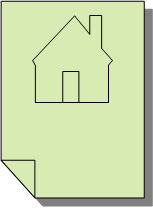
\includegraphics[width=0.25\textwidth]{figures/Homepage-icon.png}
  \end{center}
  \caption{Homepage icon}
  \label{fig:homepageicon}
\end{figure}

\begin{table}[!ht]
  \begin{center}
    \caption{Configurations tested}
    \label{tab:configstested}
    \begin{tabular}{l|c} % <-- Alignments: 1st column left, 2nd middle and 3rd right, with vertical lines in between
      \textbf{Configuration} & \textbf{Description} \\
      \hline
      1 & Simple test with one server\\
      2 & Simple test with one server\\
    \end{tabular}
  \end{center}
\end{table}
\todo[inline, backgroundcolor=kth-lightblue40]{Testade konfigurationer}

\section{Implementation …/Modeling/Simulation/…}
\label{sec:implementationDetails}
\todo[inline, backgroundcolor=kth-lightblue40]{Implementering … / modellering / simulering / …}


\subsection{Some examples of coding}

Listing~\ref{lst:helloWorldInC} shows an example of a simple program written
in C code.

\begin{lstlisting}[language={C}, caption={Hello world in C code}, label=lst:helloWorldInC]
int main() {
printf("hello, world");
return 0;
}
\end{lstlisting}


In contrast, Listing~\ref{lst:programmes} is an example of code in Python to
get a list of all of the programs at KTH.

\lstset{extendedchars=true}
\begin{lstlisting}[language={Python}, caption={Using a python program to
    access the KTH API to get all of the programs at KTH}, label=lst:programmes]
KOPPSbaseUrl = 'https://www.kth.se'

def v1_get_programmes():
    global Verbose_Flag
    #
    # Use the KOPPS API to get the data
    # note that this returns XML
    url = "{0}/api/kopps/v1/programme".format(KOPPSbaseUrl)
    if Verbose_Flag:
        print("url: " + url)
    #
    r = requests.get(url)
    if Verbose_Flag:
        print("result of getting v1 programme: {}".format(r.text))
    #
    if r.status_code == requests.codes.ok:
        return r.text           # simply return the XML
    #
    return None
\end{lstlisting}


\cleardoublepage
\chapter{Results and Analysis}
\label{ch:resultsAndAnalysis}
\todo[inline, backgroundcolor=kth-lightblue40]{svensk: Resultat och Analys}

\todo[inline]{
Sometimes this is split into two chapters.\\
  
Keep in mind: How you are going to evaluate what you have done? What are your metrics?\\
Analysis of your data and proposed solution\\
Does this meet the goals which you had when you started?
}

In this chapter, we present the results and discuss them.

\todo[inline, backgroundcolor=kth-lightblue40]{I detta kapitel presenterar vi resultaten och diskutera dem.\\
Ibland delas detta upp i två kapitel.\\
Hur du ska utvärdera vad du har gjort? Vad är din statistik?\\
Analys av data och föreslagen lösning\\
Innebär detta att uppfyllelse av de mål som du hade när du började?
}

\section{Major results}
\todo[inline, backgroundcolor=kth-lightblue40]{Huvudsakliga resultat}

Some statistics of the delay measurements are shown in Table~\ref{tab:delayMeasurements}.
The delay has been computed from the time the GET request is received until the response is sent.

\todo[inline, backgroundcolor=kth-lightblue40]{Lite statistik av fördröjningsmätningarna visas i Tabell~\ref{tab:delayMeasurements}. Förseningen har beräknats från den tidpunkt då begäran GET tas emot fram till svaret skickas.}

\begin{table}[!ht]
  \begin{center}
    \caption{Delay measurement statistics}
    \label{tab:delayMeasurements}
    \begin{tabular}{l|S[table-format=4.2]|S[table-format=3.2]} % <-- Alignments: 1st column left, 2nd middle and 3rd right, with vertical lines in between
      \textbf{Configuration} & \textbf{Average delay (ns)} & \textbf{Median delay (ns)}\\
      \hline
      1 & 467.35 & 450.10\\
      2 & 1687.5 & 901.23\\
    \end{tabular}
  \end{center}
\end{table}

Table \ref{tab:ping_results} shows the measurement of round trip times from four hosts to and from a server.
\begin{table}[ht!]
\caption[RTT for 4 hosts]{Result for the ping measurements of RTT for 4 hosts} 
\label{tab:ping_results}
\vspace{1em}
\centering
\begin{tabular}{l *{4}{S[table-format=2.3]}}
{} & \multicolumn{4}{c}{host to server RTT in ms} \\
\cmidrule{2-5}
Host & \multicolumn{1}{c}{min}  & \multicolumn{1}{c}{avg} & \multicolumn{1}{c}{max} & \multicolumn{1}{c}{mdev} \\
\midrule
h1 & 5.625 & 5.625 & 5.625 & 0.0 \\
h2 & 2.909 & 2.909 & 1.909 & 0.0 \\
h3 & 5.007 & 5.007 & 5.007 & 0.0 \\
h4 & 2.308 & 2.308 & 2.308 & 0.0 \\
\midrule
\end{tabular}
\end{table}
\FloatBarrier

\todo[inline, backgroundcolor=kth-lightblue40]{Fördröj mätstatistik}
\todo[inline, backgroundcolor=kth-lightblue40]{Konfiguration | Genomsnittlig fördröjning (ns) | Median fördröjning (ns)}

Figure \ref{fig:processing_vs_payload_length} shows and example of the
performance as measured in the experiments.

\begin{figure}[!ht]
% GNUPLOT: LaTeX picture
\setlength{\unitlength}{0.240900pt}
\ifx\plotpoint\undefined\newsavebox{\plotpoint}\fi
\begin{picture}(1500,900)(0,0)
\sbox{\plotpoint}{\rule[-0.200pt]{0.400pt}{0.400pt}}%
\put(171.0,131.0){\rule[-0.200pt]{4.818pt}{0.400pt}}
\put(151,131){\makebox(0,0)[r]{ 1.5}}
\put(1419.0,131.0){\rule[-0.200pt]{4.818pt}{0.400pt}}
\put(171.0,212.0){\rule[-0.200pt]{4.818pt}{0.400pt}}
\put(151,212){\makebox(0,0)[r]{ 2}}
\put(1419.0,212.0){\rule[-0.200pt]{4.818pt}{0.400pt}}
\put(171.0,292.0){\rule[-0.200pt]{4.818pt}{0.400pt}}
\put(151,292){\makebox(0,0)[r]{ 2.5}}
\put(1419.0,292.0){\rule[-0.200pt]{4.818pt}{0.400pt}}
\put(171.0,373.0){\rule[-0.200pt]{4.818pt}{0.400pt}}
\put(151,373){\makebox(0,0)[r]{ 3}}
\put(1419.0,373.0){\rule[-0.200pt]{4.818pt}{0.400pt}}
\put(171.0,454.0){\rule[-0.200pt]{4.818pt}{0.400pt}}
\put(151,454){\makebox(0,0)[r]{ 3.5}}
\put(1419.0,454.0){\rule[-0.200pt]{4.818pt}{0.400pt}}
\put(171.0,534.0){\rule[-0.200pt]{4.818pt}{0.400pt}}
\put(151,534){\makebox(0,0)[r]{ 4}}
\put(1419.0,534.0){\rule[-0.200pt]{4.818pt}{0.400pt}}
\put(171.0,615.0){\rule[-0.200pt]{4.818pt}{0.400pt}}
\put(151,615){\makebox(0,0)[r]{ 4.5}}
\put(1419.0,615.0){\rule[-0.200pt]{4.818pt}{0.400pt}}
\put(171.0,695.0){\rule[-0.200pt]{4.818pt}{0.400pt}}
\put(151,695){\makebox(0,0)[r]{ 5}}
\put(1419.0,695.0){\rule[-0.200pt]{4.818pt}{0.400pt}}
\put(171.0,776.0){\rule[-0.200pt]{4.818pt}{0.400pt}}
\put(151,776){\makebox(0,0)[r]{ 5.5}}
\put(1419.0,776.0){\rule[-0.200pt]{4.818pt}{0.400pt}}
\put(171.0,131.0){\rule[-0.200pt]{0.400pt}{4.818pt}}
\put(171,90){\makebox(0,0){ 0}}
\put(171.0,756.0){\rule[-0.200pt]{0.400pt}{4.818pt}}
\put(298.0,131.0){\rule[-0.200pt]{0.400pt}{4.818pt}}
\put(298,90){\makebox(0,0){ 10}}
\put(298.0,756.0){\rule[-0.200pt]{0.400pt}{4.818pt}}
\put(425.0,131.0){\rule[-0.200pt]{0.400pt}{4.818pt}}
\put(425,90){\makebox(0,0){ 20}}
\put(425.0,756.0){\rule[-0.200pt]{0.400pt}{4.818pt}}
\put(551.0,131.0){\rule[-0.200pt]{0.400pt}{4.818pt}}
\put(551,90){\makebox(0,0){ 30}}
\put(551.0,756.0){\rule[-0.200pt]{0.400pt}{4.818pt}}
\put(678.0,131.0){\rule[-0.200pt]{0.400pt}{4.818pt}}
\put(678,90){\makebox(0,0){ 40}}
\put(678.0,756.0){\rule[-0.200pt]{0.400pt}{4.818pt}}
\put(805.0,131.0){\rule[-0.200pt]{0.400pt}{4.818pt}}
\put(805,90){\makebox(0,0){ 50}}
\put(805.0,756.0){\rule[-0.200pt]{0.400pt}{4.818pt}}
\put(932.0,131.0){\rule[-0.200pt]{0.400pt}{4.818pt}}
\put(932,90){\makebox(0,0){ 60}}
\put(932.0,756.0){\rule[-0.200pt]{0.400pt}{4.818pt}}
\put(1059.0,131.0){\rule[-0.200pt]{0.400pt}{4.818pt}}
\put(1059,90){\makebox(0,0){ 70}}
\put(1059.0,756.0){\rule[-0.200pt]{0.400pt}{4.818pt}}
\put(1185.0,131.0){\rule[-0.200pt]{0.400pt}{4.818pt}}
\put(1185,90){\makebox(0,0){ 80}}
\put(1185.0,756.0){\rule[-0.200pt]{0.400pt}{4.818pt}}
\put(1312.0,131.0){\rule[-0.200pt]{0.400pt}{4.818pt}}
\put(1312,90){\makebox(0,0){ 90}}
\put(1312.0,756.0){\rule[-0.200pt]{0.400pt}{4.818pt}}
\put(1439.0,131.0){\rule[-0.200pt]{0.400pt}{4.818pt}}
\put(1439,90){\makebox(0,0){ 100}}
\put(1439.0,756.0){\rule[-0.200pt]{0.400pt}{4.818pt}}
\put(171.0,131.0){\rule[-0.200pt]{0.400pt}{155.380pt}}
\put(171.0,131.0){\rule[-0.200pt]{305.461pt}{0.400pt}}
\put(1439.0,131.0){\rule[-0.200pt]{0.400pt}{155.380pt}}
\put(171.0,776.0){\rule[-0.200pt]{305.461pt}{0.400pt}}
\put(30,453){\rotatebox{-270}{\makebox(0,0){Processing time (ms)}}}
\put(805,29){\makebox(0,0){Payload size (bytes)}}
\put(868.0,131.0){\rule[-0.200pt]{0.400pt}{84.074pt}}
\put(995.0,131.0){\rule[-0.200pt]{0.400pt}{98.287pt}}
\put(1173.0,131.0){\rule[-0.200pt]{0.400pt}{118.041pt}}
\put(1325.0,131.0){\rule[-0.200pt]{0.400pt}{134.904pt}}
\put(1350.0,131.0){\rule[-0.200pt]{0.400pt}{137.795pt}}
\put(1439.0,131.0){\rule[-0.200pt]{0.400pt}{155.380pt}}
\end{picture}
\caption[A GNUplot figure]{Processing time vs. payload length}\vspace{0.5cm}
\label{fig:processing_vs_payload_length}
\end{figure}
		

Given these measurements, we can calculate our processing bit rate as the inverse of the time it takes to process an additional byte divided by 8 bits per byte:

\[
	\text{bit rate} = \frac{1}{\frac{time_{byte}}{8}} = 20.03 \quad kb/s
\] 

\section{Reliability Analysis}
\todo[inline, backgroundcolor=kth-lightblue40]{Analys av tillförlitlighet\\
Tillförlitlighet i metod och data}

\section{Validity Analysis}
\todo[inline, backgroundcolor=kth-lightblue40]{Analys av validitet\\
Validitet i metod och data}

\cleardoublepage
\chapter{Discussion}
\label{ch:discussion}
\todo[inline, backgroundcolor=kth-lightblue40]{Diskussion\\
Förbättringsförslag?}
\todo[inline]{This can be a separate chapter or a section
  in the previous chapter.}

\cleardoublepage
\chapter{Conclusions and Future work}
\label{ch:conclusionsAndFutureWork}
\todo[inline, backgroundcolor=kth-lightblue40]{Slutsats och framtida arbete}

\todo[inline]{Add text to introduce the subsections of this chapter.}

\section{Conclusions}
\label{sec:conclusions}
\todo[inline, backgroundcolor=kth-lightblue40]{Slutsatser}
\todo[inline]{Describe the conclusions (reflect on the whole introduction given in Chapter 1).}


  
\todo[inline]{Discuss the positive effects and the drawbacks.\\
Describe the evaluation of the results of the degree project.\\
Did you meet your goals?\\
What insights have you gained?\\
What suggestions can you give to others working in this area?\\
If you had it to do again, what would you have done differently?}

\todo[inline, backgroundcolor=kth-lightblue40]{Uppfyllde du dina mål?\\
Vilka insikter har du fått?\\
Vilka förslag kan du ge till andra som arbetar inom detta område?
Om du skulle göra detta igen, vad skulle du ha gjort annorlunda?}

\section{Limitations}
\label{sec:limitations}
\todo[inline, backgroundcolor=kth-lightblue40]{Begränsande faktorer\\
Vad gjorde du som begränsade dina ansträngningar? Vilka är begränsningarna i dina resultat?}
\todo[inline]{What did you find that limited your
  efforts? What are the limitations of your results?}


\section{Future work}
\label{sec:futureWork}
\todo[inline, backgroundcolor=kth-lightblue40]{Vad du har kvar ogjort?\\
Vad är nästa självklara saker som ska göras?\\
Vad tips kan du ge till nästa person som kommer att följa upp på ditt arbete?
\todo[inline]{Describe valid future work that you or someone else could or should do.\\
Consider: What you have left undone? What are the next obvious things to be done? What hints can you give to the next person who is going to follow up on your work?
}

}


Due to the breadth of the problem, only some of the initial goals have been
met. In these section we will focus on some of the remaining issues that
should be addressed in future work. ...

\subsection{What has been left undone?}
\label{what-has-been-left-undone}

The prototype does not address the third requirment, i.e., a yearly
unavailability of less than 3 minutes, this remains an open problem. ...

\subsubsection{Cost analysis}

The current prototype works, but the performance from a cost perspective makes
this an impractical solution. Future work must reduce the cost of this
solution, to do so a cost analysis needs to first be done. ...

\subsubsection{Security}

A future research effort is needed to address the security holes that results
from using a self-signed certificate. Page filling text mass. Page filling
text mass. ...


\subsection{Next obvious things to be done}

In particular, the author of this thesis wishes to point out xxxxxx remains as
a problem to be solved. Solving this problem is the next thing that should be
done. ...

\section{Reflections}
\label{sec:reflections}
\todo[inline, backgroundcolor=kth-lightblue40]{Reflektioner}
\todo[inline, backgroundcolor=kth-lightblue40]{Vilka är de relevanta ekonomiska, sociala, miljömässiga och etiska aspekter av ditt arbete?}
\todo[inline]{What are the relevant economic, social,
  environmental, and ethical aspects of your work?
}



One of the most important results is the reduction in the amount of
energy required to process each packet while at the same time reducing the
time required to process each packet.

The thesis contributes to the \gls{UN}\enspace\glspl{SDG} numbers 1 and 9 by
xxxx. 




\noindent\rule{\textwidth}{0.4mm}
\todo[inline]{In the references, let Zotero or other tool fill this
  in for you. I suggest an extended version of the IEEE  style, to include
  URLs, DOIs, ISBNs, etc., to make it easier for your reader to find
  them. This will make life easier for your opponents and examiner. \\

  IEEE Editorial Style Manual: \url{https://www.ieee.org/content/dam/ieee-org/ieee/web/org/conferences/style_references_manual.pdf}
}
\todo[inline, backgroundcolor=kth-lightblue40]{Låt Zotero eller annat verktyg fylla i det här för dig. Jag föreslår en utökad version av IEEE stil - att inkludera webbadresser, DOI, ISBN etc. - för att göra det lättare för läsaren att hitta dem. Detta kommer att göra livet lättare för dina opponenter och examinator.}

\cleardoublepage
% Print the bibliography (and make it appear in the table of contents)
\renewcommand{\bibname}{References}
\addcontentsline{toc}{chapter}{References}

\ifbiblatex
    %\typeout{Biblatex current language is \currentlang}
    \printbibliography[heading=bibintoc]
\else
    \bibliography{references}
\fi




\cleardoublepage
\appendix
\renewcommand{\chaptermark}[1]{\markboth{Appendix \thechapter\relax:\thinspace\relax#1}{}}
\chapter{Something Extra}
\todo[inline, backgroundcolor=kth-lightblue40]{svensk: Extra Material som Bilaga}

\section{Just for testing KTH colors}
\ifdigitaloutput
    \textbf{You have selected to optimize for digital output}
\else
    \textbf{You have selected to optimize for print output}
\fi
\begin{itemize}[noitemsep]
    \item Primary color
    \begin{itemize}
    \item \textcolor{kth-blue}{kth-blue \ifdigitaloutput
    actually Deep sea
    \fi} {\color{kth-blue} \rule{0.3\linewidth}{1mm} }\\

    \item \textcolor{kth-blue80}{kth-blue80} {\color{kth-blue80} \rule{0.3\linewidth}{1mm} }\\
\end{itemize}

\item  Secondary colors
\begin{itemize}[noitemsep]
    \item \textcolor{kth-lightblue}{kth-lightblue \ifdigitaloutput
    actually Stratosphere
    \fi} {\color{kth-lightblue} \rule{0.3\linewidth}{1mm} }\\

    \item \textcolor{kth-lightred}{kth-lightred \ifdigitaloutput
    actually Fluorescence\fi} {\color{kth-lightred} \rule{0.3\linewidth}{1mm} }\\

    \item \textcolor{kth-lightred80}{kth-lightred80} {\color{kth-lightred80} \rule{0.3\linewidth}{1mm} }\\

    \item \textcolor{kth-lightgreen}{kth-lightgreen \ifdigitaloutput
    actually Front-lawn\fi} {\color{kth-lightgreen} \rule{0.3\linewidth}{1mm} }\\

    \item \textcolor{kth-coolgray}{kth-coolgray \ifdigitaloutput
    actually Office\fi} {\color{kth-coolgray} \rule{0.3\linewidth}{1mm} }\\

    \item \textcolor{kth-coolgray80}{kth-coolgray80} {\color{kth-coolgray80} \rule{0.3\linewidth}{1mm} }
\end{itemize}
\end{itemize}

\textcolor{black}{black} {\color{black} \rule{\linewidth}{1mm} }



% \newacronym[⟨options⟩]{⟨label⟩}{⟨abbrv⟩}{⟨long⟩}
%\newglossaryentry{⟨label⟩}{type=\acronymtype,
%name={⟨abbrv⟩},
%description={⟨long⟩},
%text={⟨abbrv⟩},
%first={⟨long⟩ (⟨abbrv⟩)},
%plural={⟨abbrv⟩s},
%firstplural={⟨long⟩s (⟨abbrv⟩s)},
%⟨options⟩}

%\newacronym{API}{API}{Application Programming Interface}
\newglossaryentry{tld:API}{type=readme,
name={API},
description={Application Programming Interface},
text={API},
first={Application Programming Interface (API)},
plural={APIs},
firstplural={Application Programming Interfaces (APIs)},
}
\newglossaryentry{tld:DiVA}{type=readme, name={DiVA}, description={Digitala Vetenskapliga Arkivet},
first={Digitala Vetenskapliga Arkivet (DiVA)}}
\newglossaryentry{tld:IMRAD}{type=readme, name={IMRAD}, description={Introduction, Methods, Results, and Discussion},
first={Introduction, Methods, Results, and Discussion (IMRAD)}}
\newglossaryentry{tld:JSON}{type=readme, name={JSON}, description={JavaScript Object Notation},
first={JavaScript Object Notation (JSON)}}
\newglossaryentry{tld:KOPPS}{type=readme, name={KOPPS}, description={Kurs- och programplaneringssystemet},
first={Kurs- och programplaneringssystemet (KOPPS)}}
\newglossaryentry{tld:KTH}{type=readme, name={KTH}, description={KTH Royal Institute of Technology},
first={KTH Royal Institute of Technology (KTH)}}
\newglossaryentry{tld:LADOK}{type=readme, name={LADOK}, description={Lokalt adb–baserat dokumentationssystem},
first={Lokalt adb–baserat dokumentationssystem (LADOK)}}
\newglossaryentry{tld:TIMTM}{type=readme, name={TIMTM}, description={Interactive Media Technology}
first={Interactive Media Technology (TIMTM)}}
\newglossaryentry{tld:TMMTM}{type=readme, name={TMMTM}, description={Media Management}
first={Media Management (TMMTM)}}


\lstdefinestyle{latexExample}{
language=[LaTeX]{TeX},
    breaklines=true,
    postbreak=\mbox{\textcolor{red}{$\hookrightarrow$}\space},
    basicstyle=\small\tt,
    keywordstyle=\color{blue}\sf,
    identifierstyle=\color{magenta},
    commentstyle=\color{cyan},
    backgroundcolor=\color{yellow!15},
    tabsize=2,
    columns=flexible,
}
\lstset{style=latexExample}
\newcommand{\dname}[1]{\textbf{#1}}
\newcommand{\fname}[1]{\footnotesize \texttt{#1}}

\chapter{README and notes about the template}

\glsresetall[readme]
This document, written by Gerald Q. Maguire Jr,  describes the thesis template that I have developed for use at \gls{tld:KTH} and provides some background about why it is the way that it is. It is important to note that the template is \textbf{not prescriptive}, as not every thesis will have all of the parts that the template shows. However, if there is something that you decide to leave out, you should make a conscious decision to do so and you should consider the impact this may have on your thesis being approved by the examiner.

Fundamental to the design of the template are several key factors:
\begin{itemize}
    \item Helping students be successful in their degree project,
    \item Helping students produce a high-quality thesis, and
    \item Supporting all of the (relevant) phases of the degree project process.
\end{itemize}

There are several thousand theses written each year by \gls{tld:KTH} students. Every approved thesis will be entered into \gls{tld:DiVA} (independent of whether the full text is made available via \gls{tld:DiVA}). Collecting the data necessary for \gls{tld:DiVA} was a major driving force in the design of the template. This data is useful for many of the phases of the degree project, such as announcing the oral presentation.
    
This template is \textbf{not} designed for use by \gls{tld:TIMTM} and \gls{tld:TMMTM} students - as students in these two programmes are using a different structure for their reports (there is another template available for them).

\textbf{This document is a work in progress.}

\section{Introduction}
This template evolved (radically) from an earlier thesis template that was widely used at \gls{tld:KTH}. The direction of this evolution was based on the DOCX template that was developed over many years for use with students for whom I was the examiner and/or supervisor. The suggested structure and contents of the thesis reflect my experience as an examiner for more that 570 degree projects and the experience I have had as a teacher and examiner for the course II2202 Research Methodology and Scientific Writing. The template also reflects my interest as a member of KTH's Language Committee in facilitating the parallel use of English and Swedish at \gls{tld:KTH}, as well as supporting other languages. The latter aspect
reflects my experience with double degree students, who often need to have at least the abstract of their thesis available in the language(s) of their home university. The thesis template also reflects
my experience in entering the metadata for hundreds of theses into \gls{tld:DiVA} and announcing a very large number of degree project seminars.

\Cref{sec:expectedUsers} describes a number of different groups of users and how the template is relevant to them.

There were several major thoughts influencing the design of this template:
\begin{enumerate}[leftmargin=*, label=\textbf{Thought \arabic*}, ref={Thought \arabic*}]
    \item \label{thought:helpStudent} The template should help a student be successful in their degree project and help them produce a high-quality thesis in conjunction with their degree project.
    
    \item \label{thought:process} The template should help support all of the (relevant) phases of the degree project process.
    
    \item \label{thought:reducingDataEntry} Redundant data entry should be minimized in order to increase consistency.
    
    \item \label{thought:volume} There are several thousand theses written each year at \gls{tld:KTH}. In fact, theses are the second most common type of publication at \gls{tld:KTH}.
    
    \item \label{thought:inDiVA} Every approved thesis will have at least its meta data entered into \gls{tld:DiVA}. \gls{tld:DiVA} features multi-language support for title, subtitle, abstract, and keywords.
\end{enumerate}

\section{Deliminations}

This template is \textbf{not} designed for use by \gls{tld:TIMTM} and Media Management \gls{tld:TMMTM} students - as students in these two programmes are using a different structure for their reports (there is another template available for them).

Additionally, I have been told by one of my colleagues in applied mathematics that theses in this area generally do not follow the \gls{tld:IMRAD} structure.

Some parts of the template are conditional based on the value of a switch: \texttt{\textbackslash ifinswedish}. The idea is to easily have a single template that supports theses written in English or Swedish. However, in many places the conditional has not been used, but could be. Examples of this include the Swedish names for chapters and sections. Generally this information is in a note after the English chapter or section name. More complete implementation of the use of this condition remains as future work.

The template does not fully support the G5 paper format. In particular the \gls{tld:KTH} cover (produced with \texttt{\textbackslash kthcover)} and back cover (produced with \texttt{\textbackslash kthbackcover)}) have only been adapted for A4 paper. Support for G5 paper remains as future work.

The handling of the subject area (Swedish: Område för examensarbete) is currently incomplete and remains as future work. Personally, I'm still struggling to understand the rules and how one knows what the correct values are (especially for cases of \first dual degrees and \second combinations of technical subjects and education degrees).

\section{Structure of the files for the template}
Table~\ref{tab:file_structure} shows structure of the files for the template. These files are generally taken either from an existing Overleaf project, a ZIP file, or a github.

One hope is that by automatically extracting information from various sources, this information is more likely to be \textit{correct} and \textit{consistent} (supporting \ref{thought:reducingDataEntry}). This approach has been used to generate two of the files used for the template. These files are:
\begin{enumerate}
    \item The file \fname{custom\_configuration.tex} contains macros and values for configuring a project. These values are generally expected to be known at the start of the project, \eg author(s), supervisor(s). examiner, course code for the degree project program code, \etc. While this file can be manually edited, it was designed to be generate by a program that I have written that extracts most of the data from the Canvas course being used in conjunction with the degree project. One of goals of using such a program is to automatically extract data from Canvas, the \gls{tld:KTH} profile \gls{tld:API}, \gls{tld:KOPPS}, and other sources. The macros for defining this information are described in Sections \ref{sec:authorMacros}, \ref{sec:supervisorMacros}, and \ref{sec:examinerMacros} - for authors, supervisors, and examiner (respectively).

    \item The file \texttt{schools\_and\_programs.ins} contains the English and Swedish names of schools and the programs. This information was extracted by a program from \gls{tld:KOPPS}.
\end{enumerate}

We will assume that these files have been generated by someone. Later we will examine who this someone might be for each of these files.

\begin{table}[!ht]
    \caption{Structure of files for the template}
    \label{tab:file_structure}
    \small{
    \begin{tabular}{l l p{4cm}<{\raggedright}}
%\textbf{Top level} & \textbf{2\textsuperscript{nd} level} & \textbf{Description} \\
\hline
\dname{bibstyle} & \multicolumn{2}{c}{\textbf{directory containing files related to the style of the bibliography}} \\
{} & \fname{myIEEEtran.bst} & a bibtex style file  \\
\hline
\dname{figures} & \multicolumn{2}{c}{\textbf{directory containing files for figures}} \\
\hline
\dname{lib} & \multicolumn{2}{c}{\textbf{directory containing various library files}}  \\

& \fname{acronyms.tex} & a place to define the acronyms that will or might be used \\

& \fname{defines.tex} & some generally useful defines \\

& \fname{includes-after-hyperref.tex} & a special include file for packages that have to be included \textbf{after} the hyperref package \\

& \fname{includes.tex} & a centralized place to include packages that might be useful \\

& \fname{kthcolors.tex} & defines a number of colors from the \gls{tld:KTH} palette \\

& \fname{pdf\_related\_includes.tex} & includes to be able to add the title and other information to the PDF file \\

& \fname{schools\_and\_programs.ins} & English and Swedish names of schools and the programs \\
\hline
\fname{custom\_configuration.tex} & & macros and values for configuring a project\\

\fname{examplethesis.tex} & & an example of the thesis itself \\

\fname{kth\_logo.png} & & the \gls{tld:KTH} logo for use on the cover \\

\fname{kththesis.cls} & & the kththesis class file \\

\fname{README\_notes.tex} & & these notes \\

\fname{references.bib} & & references that may be cited in the thesis \\
    \end{tabular}
    }
\end{table}
%\FloatBarrier
\clearpage


\section{Expected users and their differences}
\label{sec:expectedUsers}
This template is relevant to a number of different sets of users:
\begin{enumerate}[leftmargin=*,label=\textbf{Users \arabic*}, ref={Users \arabic*}]
    \item \label{users:authors} Author or Authors (see \Cref{sec:authors}),
    \item \label{users:others} Those working together with the author(s) during the degree project process (see \Cref{sec:examinerAdvisorsOpponent}),
    \item \label{users:admins} Administrative staff working with the document after it has been approved by the examiner (see \Cref{sec:adminStaff}), and
    \item \label{users:readers} The (hopefully) many (human) readers of the final document (see \Cref{sec:readers}).
    \item \label{users:searchEngines} The (hopefully) many computers reading the metadata and the full text of the final document (see \Cref{sec:searchEngines}).
    \item \label{users:maintainer} Those who are maintaing or updating this template (see \Cref{sec:maintainer}).
\end{enumerate}

Each of these different sets of users have different needs and perspectives. The following subsections describe these needs and perspectives.

\section{Author or Authors}
\label{sec:authors}
One of the hardest problems an author faces is getting started writing, i.e., the blank sheet of paper - empty file barrier. The template provides a non-blank starting point; hence, avoiding the blank paper barrier. Additionally, the template provides some initial structure, basically an  \gls{tld:IMRAD} structure, so that there are hints of were to place material. Moreover, there are places (and notes) about material that the student should consider adding; for example, the ``required reflections'' section in the final chapter.

The template also provides some examples of commonly occurring types of content, so that one can easily find examples of how to include a figure, table, code listing, etc. These examples are not meant to be exhaustive and quite often the student will probably need to learn new \LaTeX\ commands in the course of writing their thesis.

\subsection{Author configuration of the template}
\label{sec:authorConfigs}
The template is designed to handle a thesis written in English or Swedish.
You can set the default language to `english' or `swedish' by passing an option to the documentclass. Note that the language options is written in all lower case letters; for example, to set the document's language to English:
\begin{lstlisting}
\documentclass[english]{kththesis}
\end{lstlisting}

To set the document's language to Swedish:
\begin{lstlisting}
\documentclass[swedish]{kththesis}
\end{lstlisting}

The language option `swedish' sets the conditional \texttt{\textbackslash ifinswedish} to true.  Among many other things, this conditional is used to configure the \gls{tld:KTH} cover and the title page to use the chosen language.

The two most common bibliographic engines are supported, \ie BibTeX and BibLaTeX. To set the language to English and use the bibliographic engine to BibTeX you would say:
\begin{lstlisting}
\documentclass[english, bibtex]{kththesis}
\end{lstlisting}
To set the language to Swedish and use the bibliographic engine to BibLaTeX you would say:
\begin{lstlisting}
\documentclass[swedish, biblatex]{kththesis}
\end{lstlisting}

The above illustrates that you can pass multiple options to the document class separated by commas. Also note that the options were passed as all lower case letters.

You can of course also modify the formatting of the citations and bibliography. See for example the following code snippet:
\small{
\begin{lstlisting}
\ifbiblatex
    %\usepackage[language=english,bibstyle=authoryear,citestyle=authoryear, maxbibnames=99]{biblatex}
    %\usepackage[style=numeric,sorting=none,backend=biber]{biblatex}
    \usepackage[bibstyle=authoryear,citestyle=authoryear, maxbibnames=99,language=english]{biblatex}
    % alternatively you might use another style, such as IEEE
    %\usepackage[style=ieee]{biblatex}
    \addbibresource{references.bib}
    %\DeclareLanguageMapping{norsk}{norwegian}
\else
    % The line(s) below are for BibTeX
    \bibliographystyle{bibstyle/myIEEEtran}
    %\bibliographystyle{apalike}
\fi
\end{lstlisting}
}

To optimize for digital output (this changes the color palette) add the option: digitaloutput. There are also options for A4 or G6 paper: a4paper or g5paper (respectively). Finally, there are options for a 1\textsuperscript{st} cycle thesis or 2\textsuperscript{nd} cycle thesis: bachelor and master (respectively).

One of the first things that the author(s) will want to do is add the working title and subtitle to the thesis. This is done using the \textbackslash title, \textbackslash subtitle, \textbackslash alttitle, and \textbackslash altsubtitle macros as shown below:
\begin{lstlisting}
\title{This is the title in the language of the thesis}
\subtitle{An subtitle in the language of the thesis}

% give the alternative title - i.e., if the thesis is in English, then give a Swedish title
\alttitle{Detta är den svenska översättningen av titeln}
\altsubtitle{Detta är den svenska översättningen av undertiteln}
% alternative, if the thesis is in Swedish, then give an English title
%\alttitle{This is the English translation of the title}
%\altsubtitle{This is the English translation of the subtitle}   
\end{lstlisting}

Setting these values once and then using them in many places reduces the work to change them while at the same time ensuring consistency. 

Some additional configuration that the author(s) might do is to set the values of the macros related to the course cycle, course code, date of the thesis, number of credits, degree/exam name, subject area, and if the degree is done external to \gls{tld:KTH} to set the host information. Consider the snippet below for a student admitted to the ``Bachelor's Programme in Information and Communication Technology (TCOMK)'' program and enrolled in the degree project course ``IA150X Degree Project in Information and Communication Technology, First Cycle 15.0 credits'' and a company ``Företaget AB'':
\begin{lstlisting}
\hostcompany{Företaget AB} % Remove this line if the project was not done at a host company

\date{\today}

\courseCycle{1}
\courseCode{IA150X}
\courseCredits{15.0}

\programcode{TCOMK}
\degreeName{Bachelors degree}
% Note that the subject area for a Bachelor's thesis (Kandidatexamen)
% should be either Technology or Architecture
% If the thesis is in Swedish these would be: teknik | arkitektur
% -- Note the use of lower case for the Swedish subject area
\subjectArea{Technology}
\end{lstlisting}

Note that in the above macros you have to give the English or Swedish names in the arguments to \textbackslash degreeName and \textbackslash subjectArea - as shown below:
\begin{lstlisting}
\degreeName{Kandidatexamen}
\subjectArea{teknik}
\end{lstlisting}

For a CDATE student enrolled in the course ``DA231X Degree Project in Computer Science and Engineering, Second Cycle 30.0 credits'', the cycle, program, course code, degree, and subject area information would be:
\begin{lstlisting}
\programcode{CDATE}
\courseCycle{2}
\courseCode{DA231X}
\courseCredits{30.0}
\degreeName{Degree of Master of Science in Engineering}
\subjectArea{Computer Science and Engineering}
\end{lstlisting}

There are a set of rules about what is to be displayed on the \gls{tld:KTH} cover. These can be found at \url{https://www.kth.se/social/group/sprakkommitten/page/omrade-for-examensarbete/}.

National subject categories are a required field in the \gls{tld:DiVA} record. These categories follow a definition by SCB and HSV. 
While these code refer to research areas, these codes are also used in \gls{tld:KTH} to indicate the area of the thesis. The guidance that I received from the Linköping library was that one should try to use 5 digit codes when possible. Some examples of these codes are shown in Table~\ref{tab:nationalsubject categories}.
\begin{description}[leftmargin=!, labelwidth =\widthof{\texttt{\textbackslash nationalsubjectcategories\{\}}}]
\item [\texttt{\textbackslash nationalsubjectcategories\{\}}] comma separated list of national subject category codes - each a 3 or 5 digit code
\end{description}

An example for a thesis in Computer Science and Computer Systems:
\begin{lstlisting}
\nationalsubjectcategories{10201, 10206}
\end{lstlisting}

You can find the subjects and their codes in:\\ \url{https://www.scb.se/contentassets/3a12f556522d4bdc887c4838a37c7ec7/standard-for-svensk-indelning--av-forskningsamnen-2011-uppdaterad-aug-2016.pdf}\\
and\\
\url{https://www.scb.se/contentassets/10054f2ef27c437884e8cde0d38b9cc4/oversattningsnyckel-forskningsamnen.pdf}

\begin{table}[!ht]
  \begin{center}
    \caption{Examples of some national subject categories and their codes}
    \label{tab:nationalsubject categories}
    \begin{tabular}{p{0.85cm} L{6.2cm} L{6.2cm}} % <-- Alignments: 1st column left, 2nd middle, with vertical lines in between
      \textbf{Code}  & \textbf{Category (in Swedish)} & \textbf{Category (in English)} \\
      \hline
102 & Data- och informationsvetenskap (Datateknik) &   Computer and Information Sciences \\
      \hline
10201 & Datavetenskap (datalogi) & Computer Sciences \\
      \hline
10202 & Systemvetenskap, informationssystem och informatik (samhällsvetenskaplig inriktning under 50804) &
Information Systems (Social aspects to be 50804)\\
      \hline
10203 & Bioinformatik (beräkningsbiologi) (tillämpningar under 10610) & Bioinformatics (Computational Biology) (applications to be 10610) \\
      \hline
10204 & Människa-datorinteraktion (interaktionsdesign) (Samhällsvetenskapliga aspekter under 50803) & Human Computer Interaction (Social aspects to be 50803)\\
      \hline
10205 & Programvaruteknik & Software Engineering \\
      \hline
10206 & Datorteknik & Computer Engineering \\
      \hline
10207 & Datorseende och robotik (autonoma system) & Computer Vision and Robotics (Autonomous Systems) \\
      \hline
10208 & Språkteknologi (språkvetenskaplig databehandling) & Language Technology (Computational Linguistics) \\
      \hline
10209 & Medieteknik & Media and Communication Technology \\
      \hline
10299 & Annan data- och informationsvetenskap & Other Computer and Information Science \\
      \hline
      \hline
202   & Elektroteknik och elektronik & Electrical Engineering, Electronic Engineering, Information Engineering \\
      \hline
20201 & Robotteknik och automation & Robotics \\
      \hline
20202 & Reglerteknik & Control Engineering \\
      \hline
20203 & Kommunikationssystem & Communication Systems \\
      \hline
20204 & Telekommunikation & Telecommunications \\
      \hline
20205 & Signalbehandling & Signal Processing \\
      \hline
20206 & Datorsystem & Computer Systems \\
      \hline
20207 & Inbäddad systemteknik & Embedded Systems \\
      \hline
20299 & Annan elektroteknik och elektronik & Other Electrical Engineering, Electronic Engineering, Information Engineering \\
      \hline
    \end{tabular}
  \end{center}
\end{table}


\FloatBarrier

\subsection{Author configuration of the \LaTeX\ engine}
\label{sec:latexEngine}
The template should work with pdflatex, XeLaTeX, and LuaLaTeX.  If you are using Overleaf, I strongly recommend the use of XeLaTeX ---  as this will get the \texttt{Arial} fonts correct for the \gls{tld:KTH} cover. If you are running the compiler on your local machine and you use XeLaTeX \textbf{and} you have \texttt{Arial} as a system font, then it will be able to use it. Similarly, for LuaLaTeX. For pdflatex I have used \textbackslash fontfamily{helvet}, i.e., Helvetica, as it is a sans serif font.

\subsection{Author macros}
\label{sec:authorMacros}
It is assumed that there can only be 1 or 2 authors. For many years now 2\textsuperscript{nd} cycle theses are expected to only have one author.

For the author or first author, there are a number of macros defined to store information about the author, so that it can later be used in multiple places (for example, the \gls{tld:KTH} cover (produced with \texttt{\textbackslash kthcover)}, the title page (produced with \texttt{\textbackslash titlepage}, the ``For DIVA'' section at the end of the thesis (produced with 
\texttt{\textbackslash divainfo\{pg:lastPageofPreface\}\{pg:lastPageofMainmatter\}}), and possibly a file named \texttt{fordiva.json} produced as a by product of the \texttt{\textbackslash divainfo}. Note that the section name has \gls{tld:DiVA} set in all caps - which hopefully should not occur in the thesis!

The author related macros are:
\begin{description}[leftmargin=!, labelwidth =\widthof{\texttt{\textbackslash secondAuthorsFirstname\{\}}}]
\item [\texttt{\textbackslash authorsLastname\{\}}] the last name of the author

\item [\texttt{\textbackslash authorsFirstname\{\}}] the first name of the author

\item [\texttt{\textbackslash email\{\}}] the \gls{tld:KTH} e-mail address of the author

\item [\texttt{\textbackslash kthid\{\}}] the author's kthid, this generally start with the string ·``u1'' and is a unique identifier for every \gls{tld:KTH} user.

% As per email from KTH Biblioteket on 2021-06-28 students cannot have an OrCiD reported for their degree project
\item [\texttt{\textbackslash authorsSchool\{\}}] the value is generally of the form:\linebreak[4] \texttt{\textbackslash schoolAcronym\{EECS\}}. The currently supported school acronyms are: ABE, CBH, EECS, ITM, and SCI. These are defined in the file \texttt{schools\_and\_programs.ins}.
\end{description}

If the first author is not in Stockholm, Sweden when the acknowledgements are written, then add that information via the macros described below.
This information will be used when generating the acknowledgements signature. The acknowledgements signature is the text at the end of the acknowledgements and it gives the place where the author(s) is/are when writing the acknowledgements and also gives the date and name(s).
\begin{description}[leftmargin=!, labelwidth =\widthof{\texttt{\textbackslash secondAuthorsFirstname\{\}}}]
\item [\texttt{\textbackslash authorCity\{A City\}}] specify the city

\item [\texttt{\textbackslash authorCountry\{A Country\}}] specify the country

\item [\texttt{\textbackslash authorCityCountryDate\{\}}] pass into this function the month and year for the acknowledgement. This can be a string such as January 2022 or it can be a \LaTeX\ expression, such as \textbackslash MONTH\textbackslash enspace\textbackslash the\textbackslash year.
\end{description}

If there is a second author and the place, month, and year are \textbf{all} the same, then specify the month and year for only the \textbf{first} author:
\begin{lstlisting}
\authorCityCountryDate{\MONTH\enspace\the\year}
\end{lstlisting}

If there is a second author and the place is different, then say:
\begin{lstlisting}
\authorCityCountryDate{}
\end{lstlisting}

If there is a second author, the macros are:
\begin{description}[leftmargin=!, labelwidth =\widthof{\texttt{\textbackslash secondAuthorsFirstname\{\}}}]
\item [\texttt{\textbackslash secondAuthorsLastname\{\}}] the last name of the 2\textsuperscript{nd} author
\item [\texttt{\textbackslash secondAuthorsFirstname\{\}}] the first name of the 2\textsuperscript{nd} author
\item [\texttt{\textbackslash secondemail\{\}}] the \gls{tld:KTH} e-mail address of the 2\textsuperscript{nd} author
\item [\texttt{\textbackslash secondkthid\{\}}] the 2\textsuperscript{nd} author's kthid
% As per email from KTH Biblioteket on 2021-06-28 students cannot have an OrCiD reported for their degree project
\item [\texttt{\textbackslash secondAuthorsSchool\{\}}] the school of the 2\textsuperscript{nd} author
\end{description}

If the second author is not in the same place as the first author, then add the relevant information using the macros below.  This information will be used when generating the acknowledgements signature.
\begin{description}[leftmargin=!, labelwidth =\widthof{\texttt{\textbackslash secondAuthorsFirstname\{\}}}]
\item [\texttt{\textbackslash secondAuthorCity\{A City\}}]  specify the city

\item [\texttt{\textbackslash secondAuthorCountry\{A Country\}}] specify the country

\item [\texttt{\textbackslash secondAuthorCityCountryDate\{\textbackslash MONTH\textbackslash enspace\textbackslash the\textbackslash year\}}]  pass into this function the month and year for the acknowledgement
\end{description}

If the second author is the same place as the first author, then comment out or delete the \textbackslash secondAuthorCityCountryDate\{\} as shown below:
\begin{lstlisting}
%\secondAuthorCityCountryDate{}
\end{lstlisting}

\section{Those working in parallel with the authors(s) during the degree project}
\label{sec:examinerAdvisorsOpponent}
Those working together with the author(s) during the degree project process include the examiner, supervisor(s), and the opponent(s).

\subsection{Supervisor}
\label{sec:supervisorMacros}
If a degree project is done in industry, there is generally an industrial supervisor in addition to the academic supervisor(s). The template supports up to 3 supervisors (typically an academic supervisor, an industrial supervisor, and sometimes an additional academic or industrial supervisor). The choice of up to three reflects my experience and observation of prior theses in \gls{tld:DiVA}. Note that there is expected to be at least one supervisor. The supervisors are enumerated as A, B, and C. For each of A, B, and C as appropriate, replace the "X" in the following macros:
\begin{description}[leftmargin=!, labelwidth =\widthof{\texttt{\textbackslash secondAuthorsFirstname\{\}}}]
\item [\texttt{\textbackslash supervisorXsLastname\{\}}] the last name of the supervisor
\item [\texttt{\textbackslash supervisorXsFirstname\{\}}] the first name of the supervisor
\item [\texttt{\textbackslash supervisorXsEmail\{\}}] e-mail address of the supervisor
\end{description}

If the supervisor is from within \gls{tld:KTH}, then add their KTHID, School, and Department info:
\begin{description}[leftmargin=!, labelwidth =\widthof{\texttt{\textbackslash secondAuthorsFirstname\{\}}}]
\item [\texttt{\textbackslash supervisorXsKTHID\{\}}] the supervisor's kthid 
\item [\texttt{\textbackslash supervisorXsSchool\{\}}] the school of the supervisor
\item [\texttt{\textbackslash supervisorXsDepartment\{\}}] the department of the supervisor
\end{description}

If the supervisor is from outside of \gls{tld:KTH}, then add their organization with:
\begin{description}[leftmargin=!, labelwidth =\widthof{\texttt{\textbackslash secondAuthorsFirstname\{\}}}]
\item [\texttt{\textbackslash supervisorXsOrganization\{\}}] the supervisor's organization
\end{description}

\subsection{Examiner}
\label{sec:examinerMacros}
I assume that there is only a single examiner for a given thesis. For this examiner, the relevant macros are:
\begin{description}[leftmargin=!, labelwidth =\widthof{\texttt{\textbackslash secondAuthorsFirstname\{\}}}]
\item [\texttt{\textbackslash examinersLastname\{\}}] the last name of the examiner
\item [\texttt{\textbackslash examinersFirstname\{\}}] the first name of the examiner
\item [\texttt{\textbackslash examinersEmail\{\}}] e-mail address of the examiner
\end{description}

If the examiner is from within \gls{tld:KTH}, then add their KTHID, School, and Department info:
\begin{description}[leftmargin=!, labelwidth =\widthof{\texttt{\textbackslash secondAuthorsFirstname\{\}}}]
\item [\texttt{\textbackslash examinersKTHID\{\}}] the examiner's kthid 
\item [\texttt{\textbackslash examinersSchool\{\}}] the school of the examiner
\item [\texttt{\textbackslash examinersDepartment\{\}}] the department of the examiner
\end{description}

If the examiner is from outside of \gls{tld:KTH}, then add their organization with:
\begin{description}[leftmargin=!, labelwidth =\widthof{\texttt{\textbackslash secondAuthorsFirstname\{\}}}]
\item [\texttt{\textbackslash examinersOrganization\{\}}] the examiner's organization
\end{description}


I assume that someone (such as the examiner) will generate the file:\linebreak[4] \fname{custom\_configuration.tex}. This assumption is based upon the fact that the examiner knows who the student or students are who will be working in a given degree project, who the supervisor or supervisors are, what program the student is in, course code, \ldots . Ideally this file should be generated automatically by some computer program so that each student or pair of students in a group gets a customized template automatically via the Canvas course. However, currently the file is generated using a command line program (\texttt{create\_customized\_JSON\_file.py}) to generate a \gls{tld:JSON} file. Subsequently, a separate program (\texttt{customize\_LaTeX\_project.py}) takes this \gls{tld:JSON} data and create the appropriate \LaTeX\ commands and inserts this information into the file and then inserts this file into a ZIP file, either replacing or augmenting the \fname{custom\_configuration.tex} within this ZIP file (if one exists). There is an option for this second program \texttt{--initialize} that causes the program to simply replace the file rather than appending the new information to the end of the file.

The above programs are available from \url{https://github.com/gqmaguirejr/E-learning}. The README file for this github contains information about how to run the programs, their options, and gives examples.

\subsection{Opponent(s) and oral presentation}
\label{sec:opponentMacros}
Unlike the supervisors and examiner, the macros related to the opponent and oral presentation are in the \fname{examplethesis.tex} file.
The macro for the opponent(s) is: 
\begin{description}[leftmargin=!, labelwidth =\widthof{\texttt{\textbackslash secondAuthorsFirstname\{\}}}]
\item [\texttt{\textbackslash opponentsNames\{\}}] the names (in normal name order) of the opponent or opponents
\end{description}
When there are multiple opponents, separate their names with '\textbackslash \&'; for example, A. B. Normal \textbackslash \& A. X. E. Normalè.

For the oral presentation, the following macros are filled in once the examiner has scheduled your oral presentation:
\begin{description}[leftmargin=!, labelwidth =\widthof{\texttt{\textbackslash presentationDateAndTimeISO\{\}}}]
\item [\texttt{\textbackslash presentationDateAndTimeISO\{\}}] date and time of the presentation is ISO format, for example: 2022-03-15 13:00
\item [\texttt{\textbackslash presentationLanguage\{\}}] three letter abbreviation for the language of the presentation according to three letter ISO 639-2 Code – specifically the "B" (bibliographic) variant of these codes (note that this is the same language code used in DiVA), generally eng or swe
\item [\texttt{\textbackslash presentationRoom\{\}}] a room name and/or\hspace*{\fill}\linebreak[4] ``via Zoom https://kth-se.zoom.us/j/ddddddddddd''
\item [\texttt{\textbackslash presentationAddress\{\}}] location of the room, for example: Isafjordsgatan 22 (Kistagången 16)
\item [\texttt{\textbackslash presentationCity\{\}}] city where the presentation occurs, generally: Stockholm
\end{description}


\section{Administrative staff}
\label{sec:adminStaff}

Once a thesis is approved by the examiner we need to add the TRITA number. The TRITA number is assigned by the student affairs office of the school from an annual series of numbers.

\subsection{What is a TRITA number and why does each approved thesis get assigned one?}

TRITA stands for Transactions for the Royal Institute of Technology, added by the letter "A". The TRITA definition is the 1971 report, "Mall för publikationsserier vid Kungl. Tekniska högskolan i Stockholm", TRITA-LIB-1001, \url{http://urn.kb.se/resolve?urn=urn:nbn:se:kth:diva-127656}.

The format for TRITA numbers for degree projects is TRITA-$\langle$school acronym$\rangle$-EX-YYYY:nnn, where nnn is a sequential number starting from 1 each year with the numbers assigned in chronological order to approved theses ("numren delas ut kronologiskt först när examinatorn godkänt arbetet." - according to one of KTH's archivists). Note that the list of assigned TRITA numbers is itself archived each year.

The TRITA number value can be set with a macro that takes two arguments: series and year:number as shown below:
\begin{lstlisting}
% for entering the TRITA number for a thesis
\trita{TRITA-EECS-EX}{2022:00}  
\end{lstlisting}

\subsection{Where does the TRITA number go?}
The TRITA number will appear on the back cover of the thesis. It is also stored as part of the meta data that is entered into \gls{tld:DiVA}.

\subsection{What does this mean in practice?}
Currently at EECS the TRITA number is only assigned to the thesis when the examiner has approved the thesis and submitted the PDF of the approved thesis (with cover) to the student affairs office. Of course, this does not actually make a lot of sense because the back cover is already on the thesis! This means that someone in the student affairs office must either \first edit the sequential number part of the TRITA number (using some PDF tool) or \second they need to make a new back cover and replace the existing back cover. A better solution would be to inform the examiner of the TRITA number and the examiner can see that this number is inserted into the macro shown above and this can enable the number to appear on the back cover and as an added bonus be include in the meta data for \gls{tld:DiVA}.

\subsection{Entering the meta data into DiVA}
If a thesis has used this template the ``For DIVA'' page contains the meta data for \gls{tld:DiVA} and an administrator can cut an paste this data into \gls{tld:DiVA}. Alternatively, this meta data can be extracted with a program from the PDF file to produce a \gls{tld:JSON} file that can subsequently be used to create a MODS file for import into \gls{tld:DiVA}. The \LaTeX\ compiler can in many case produce a file called ``fordiva.json'' that contains the meta data.

The programs that can be used to extract data and to take a \gls{tld:JSON} file and create a MODS file are available from \url{https://github.com/gqmaguirejr/E-learning}.

Note that the import of the MODS file does not import the collaboration data, even though this is in the file. This is a limitation of the \gls{tld:DiVA} import function. Therefore, this information has to be manually entered along with uploading of the PDF file itself.

\section{(Human) Readers of the thesis}
\label{sec:readers}
Some theses have very few downloads from \gls{tld:DiVA} while some have had hundreds of thousands of downloads. Therefore, you should keep in mind that you have a wide range of human readers of your thesis. The readers include other students looking for information related to their own thesis or because they are interested in the future work that you have suggested to work on for their own degree project. Additionally, researchers who are looking for your results may find your thesis relevant to them. In many cases companies will look at theses for ideas about what the state of the art is - in a number of cases theses have been important as ``prior art'' and this invalidated patents that had been issued if the patent was submitted after the thesis became public (hence it pays to get theses public as soon as possible). Other human readers are the UKÄ review teams that exam the degree programs offered at \gls{tld:KTH}. Finally, as \gls{tld:KTH} is a public agency it is important that the general public know what is done at \gls{tld:KTH}.

\subsection{Machines reading the metadata or full text of the thesis}
\label{sec:searchEngines}
The file \fname{pdf\_related\_includes.tex} contains \LaTeX\ code that stores the title, author(s), and keyword information into the PDF document in such a way that if you ask for the properties of the PDF file you will get this data. This information makes it easier for machines to get this information from the PDF file. 

Additionally, many search engines (such as Google) mine \gls{tld:DiVA} for the meta-data and if the full text of the thesis is published via \gls{tld:DiVA} then they also process the full text of the thesis. The result is that search engines can find the content in these theses.  This is likely to increase the probability that someone will down load your thesis, if they think it is relevant to them - increasing the number of your human readers (see \Cref{sec:readers}).

\subsection{Template author and maintainers}
\label{sec:maintainer}

\gls{tld:KTH} periodically changes the cover design for theses, introduces new programs of study, eliminates programs of study, reorganizes administratively,
and faculty move between schools, departments, and divisions. It can be expected that this template will need to evolve with these changes.

For example, if there is a change in schools or programs then there needs to be changes made to the file \texttt{schools\_and\_programs.ins}. While the current file was extracted from \gls{tld:KOPPS}, the program that does this will need to be replaced because further development of \gls{tld:KOPPS} has been terminated by KTH's central IT unit which plans to transition all of this information to \gls{tld:LADOK}.

As another example, on 13 December 2021 there was a change in the \gls{tld:KTH} cover for 1\textsuperscript{st} and 2\textsuperscript{nd} theses and the cover generator web service was shutdown. The initial draft version of the cover used a proprietary font (TheSans B4 SemiLight and TheSans B6 SemiBold). The version that was publicly introduced uses another proprietary font (Arial) and officially only existed as a DOCX file for a thesis in Swedish. The result is that I had to make my own version in \LaTeX\ to try to emulate the DOCX cover. This lead to a lot of effort, but one can get a reasonable cover with the correct font as described in Section \ref{sec:latexEngine}.

\section{While writing}
As was noted in \Cref{sec:authors} the thesis contains lots of examples, notes, and comments. One method used to provide additional information is the use of \textbackslash todo.A number of different types of todo notes have been used in the thesis. These are described in \Cref{sec:todonotes}.

\subsection{Conventions for todo notes}
\label{sec:todonotes}
The example thesis text includes extensive comments, directions, and warnings. These follow the form shown below:
\begin{lstlisting}
\todo[inline]{Comments/directions/... in English}
\todo[inline, backgroundcolor=kth-lightblue40]{Text på svenska}
\todo[inline, backgroundcolor=kth-lightgreen40]{English descriptions about formatting}
\todo[inline, backgroundcolor=kth-lightred40]{warning}  
\end{lstlisting}
and appear as:
\todo[inline]{Comments/directions/... in English}
\todo[inline, backgroundcolor=kth-lightblue40]{Text på svenska}
\todo[inline, backgroundcolor=kth-lightgreen40]{English descriptions about formatting}
\todo[inline, backgroundcolor=kth-lightred40]{warning}

\subsection{Removing the README\_notes}
At some point you will no longer want this README information. You can remove it by removing the line
\textbackslash include\{README\_notes/README\_notes\} -- from the \fname{examplethesis.tex} file. You can then remove the \dname{README\_notes} directory.

\clearpage
\printglossary[type=readme,toctitle={README acronyms}]
\clearpage

%% The following label is necessary for computing the last page number of the body of the report to include in the "For DIVA" information
\label{pg:lastPageofMainmatter}

\clearpage
\kthbackcover
\fancyhead{}  % Do not use header on this extra page or pages
\section*{For DIVA}
\lstset{numbers=none} %% remove any list line numbering
\divainfo{pg:lastPageofPreface}{pg:lastPageofMainmatter}
\end{document}
